\newpage
	\section{CẤP SỐ NHÂN}
	\subsection{LÝ THUYẾT CẦN NHỚ}
	\subsubsection{Định nghĩa}
	\indam{Định nghĩa}
	\begin{dn}
	Cấp số nhân là một dãy số (hữu hạn hoặc vô hạn), trong đó kể từ số hạng thứ hai, mỗi số hạng đều bằng số hạng đứng ngay trước nó nhân với một số không đổi $q$. Nghĩa là
	$$
	\left(u_n\right) \text { là cấp số nhân } \Leftrightarrow u_n= u_{n-1}\cdot q,\quad \forall n \geq 2.
	$$
	\begin{itemize}
	\item 	Số $q$ được gọi là công bội của cấp số nhân.
	\end{itemize}
	\end{dn}
	\begin{khung4}{Đặc biệt}
	\begin{itemize}
	\item Khi $q=0$, cấp số nhân có dạng $u_1$, $0$, $0$, $0$, $\ldots$.
	\item 	Khi $q=1$, cấp số nhân có dạng $u_1$, $u_1$, $u_1$, $\ldots$.
	\end{itemize}
	\end{khung4}
	\subsubsection{Số hạng tổng quát}
	\begin{enumerate}[\iconMT]
	\item \indam{Định lí}
	\begin{dl}
	Nếu một cấp số nhân có số hạng đầu là $u_1$ và công bội $q$ thì số hạng tổng quát $u_n$ của nó tính bởi công thức
	$$u_n=u_1\cdot q^{n-1},\quad \forall n \geq 2.$$
	\end{dl}
	\end{enumerate}
	\subsubsection{Tính chất các số hạng của cấp số nhân.}
	\begin{enumerate}[\iconMT]
	\item \indam{Định lí:}
	\begin{boxdn}
	Trong một cấp số nhân, bình phương của mỗi số hạng (trừ số hạng đầu và cuối) đều là trung bình nhân của hai số hạng đứng kề với nó, nghĩa là
	$$
	u_k=\sqrt{u_{k-1} \cdot u_{k+1}} \, \text { hay } \, u_k^2=u_{k-1} \cdot u_{k+1} \, \left(k \geq 2 \right)
	$$
	\end{boxdn}
	\item \indam{Hệ quả}
	\begin{boxdn}
	Nếu $a$, $b$, $c$ là ba số khác $ 0 $, thì ba số $a$, $b$, $c$ theo thứ tự đó lập thành một cấp số nhân khi và chỉ khi $a c=b^2$.
	\end{boxdn}
	\end{enumerate}
	\subsubsection{Tổng của $ n $ số hạng đầu tiên của một cấp số cộng}
	\begin{enumerate}[\iconMT]
	\item \indam{Định lí}
	\begin{boxdn}
	Cho cấp số nhân $\left(u_n\right)$.	Đặt $S_n=u_1+u_2+\cdots+u_n$
	\begin{itemize}
	\item 	 Nếu $q=1$ thì $S_n=n\cdot u_1$.
	\item Nếu $q \neq 1$ thì $S_n=\dfrac{u_1\left(1-q^n\right)}{1-q}$.
	\end{itemize}
	\end{boxdn}
	\end{enumerate}
	%-------------------------------------------------------------------------------------------------------------
	\subsection{PHÂN LOẠI VÀ PHƯƠNG PHÁP GIẢI TOÁN}
	\begin{dang}{Bài toán xác định dãy đã cho là cấp số nhân}
	\begin{listEX}[1]
	\item Nếu $\left(u_n\right)$ là một cấp số nhân với công bội $q$ thì $u_{n+1}=u_n q$ với $n \in \mathbb{N}^*$.
	\item Để chứng minh một dãy đã cho là 1 cấp số nhân thì ta chứng minh
	$\dfrac{u_{n+1}}{u_n}=q $; $n \geq 1$ với q là một hằng số không đổi.
	\end{listEX}
	\end{dang}
	\begin{vd}
	Chứng minh các dãy số $\left(u_n\right)$ sau là cấp số nhân biết
	\begin{enumEX}{3}
	\item 	 $u_n=\dfrac{3}{5} \cdot 2^n$.
	\item $u_n=\left(-\dfrac{1}{2}\right)^n$.
	\item $u_n=(-1)^n \cdot 3^{2 n}$.
	\end{enumEX}
	\loigiai{
	\begin{enumerate}
	\item 	 $u_n=\dfrac{3}{5} \cdot 2^n$.
	\\
	Với $\forall n \in \mathbb{N}^*$, ta có $\dfrac{u_{n+1}}{u_n}=\dfrac{\dfrac{3}{5} \cdot 2^{n+1}}{\dfrac{3}{5} \cdot 2^n}=2$ không đổi.
	\\
	Suy ra dãy số $\left(u_n\right)$ là cấp số nhân với công bội bằng $2$.
	\item $u_n=\left(-\dfrac{1}{2}\right)^n$.
	\\
	Với $\forall n \in \mathbb{N}^*$, ta có $\dfrac{u_{n+1}}{u_n}=\dfrac{\left(-\dfrac{1}{2}\right)^{n+1}}{\left(-\dfrac{1}{2}\right)^n}=-\dfrac{1}{2}$ không đổi.
	\\
	Suy ra dãy số $\left(u_n\right)$ là cấp số nhân với công bội bằng $-\dfrac{1}{2}$.
	\item $u_n=(-1)^n \cdot 3^{2 n}$.
	Với $\forall n \in \mathbb{N}^*$, ta có $\dfrac{u_{n+1}}{u_n}=\dfrac{(-1)^{n+1} \cdot 3^{2(n+1)}}{(-1)^n \cdot 3^{2 n}}=-9$ không đổi.\\
	Suy ra dãy số $\left(u_n\right)$ là cấp số nhân với công bội bằng $-9$.
	\end{enumerate}
	}
	\end{vd}
	\begin{vd}
	Trong các dãy số dưới đây, dãy số nào là cấp số nhân?
	\begin{enumEX}{2}
	\item Dãy số $\left(x_n\right)$, với $x_n=n^2$.
	\item Dãy số $\left(y_n\right)$, với $y_n=\sqrt{5}^{2 n-3}$.
	\item Dãy số $\left(z_n\right)$, với $z_n=\dfrac{2}{n}$.
	\item Dãy số $\left(w_n\right)$, với $w_n=\dfrac{3^n+1}{3^{n+1}}$.
	\end{enumEX}
	\loigiai{
	\begin{enumerate}
	\item 	 Dãy số $\left(x_n\right)$, với $x_n=n^2$.
	\\
	\textbf{Cách 1.} Ba số hạng đầu của dãy số $\left(x_n\right)$ là $1$, $4$, $9$.
	\\
	Vì $4=1\cdot 4$; $9 \neq 4\cdot 4$
	\\
	Nên dãy số $\left(x_n\right)$ không phải là cấp số nhân.
	\\
	\textbf{Cách 2.} Ta có $x_{n+1}=(n+1)^2$.\\
	Nên $\dfrac{x_{n+1}}{x_n}=\dfrac{(n+1)^2}{n^2}=1+\dfrac{2}{n}+\dfrac{1}{n^2}$ (phụ thuộc vào $n$ không phải là số không đổi). \\
	Do đó, $\left(x_n\right)$ không phải là cấp số nhân.
	\item 	 Dãy số $\left(y_n\right)$, với $y_n=\sqrt{5}^{2 n-3}$.
	\\
	Ta có $y_{n+1}=(\sqrt{5})^{2(n+1)-3}=\sqrt{5}^{2 n-1}$.
	\\
	Nên $\dfrac{y_{n+1}}{y_n}=\sqrt{5}^2=5$ (là số không đổi).\\
	Do đó,, $\left(y_n\right)$ là cấp số nhân với công bội $q=5$.
	\item Dãy số $\left(z_n\right)$, với $z_n=\dfrac{2}{n}$.
	\\
	Ta có $z_{n+1}=\dfrac{2}{n+1}$.
	\\
	Nên $\dfrac{z_n+1}{z_n}=\dfrac{n}{n+1}$ (phụ thuộc vào $n$, không phải là số không đổi).
	\\
	Do đó, $\left(z_n\right)$ không phải là một cấp số nhân.
	\item Dãy số $\left(w_n\right)$, với $w_n=\dfrac{3^n+1}{3^{n+1}}$.
	\\
	Ba số hạng đầu của dãy số $\left( w _n\right)$ là $\dfrac{4}{9}$, $\dfrac{10}{27}$, $\dfrac{28}{81}$.
	\\
	Vì $\dfrac{10}{27}=\dfrac{4}{9} \cdot \dfrac{5}{6}$, $\dfrac{28}{81} \neq \dfrac{10}{27} \cdot \dfrac{5}{6}$.
	\\
	Nên dãy số $\left(w_n\right)$ không phải là cấp số nhân.
	\end{enumerate}
	}
	\end{vd}
	%-------------------------------------------------------------------------------------------------------------
	\begin{dang}{Bài toán Xác định các yếu tố qua số hạng tổng quát}
	\textbf{Phương pháp.}\\
	 Nếu một cấp số nhân có số hạng đầu là $u_1$ và công bội $q$ thì số hạng tổng quá $u_n$ của nó tính bởi công thức
	$$
	u_n=q^{n-1} \cdot u_1,\, \forall n \geq 2.
	$$
	\end{dang}
	\begin{vd}
	Cho cấp số nhân $\left(u_n\right)$ với công bội $q <0$ và $u_2=4$, $u_4=9$. Tìm $u_1$.
	\loigiai{
	Vì $q<0$, $u_2>0$ nên $u_3<0$. \\
	Do đó, $u_3=-\sqrt{u_2 \cdot u_4}=-\sqrt{4 \cdot 9}=-6$; $u_2^2=u_1 \cdot u_3 \Rightarrow u_1=\dfrac{u_2^2}{u_3}=\dfrac{4^2}{-6}=-\dfrac{8}{3}$.
	}
	\end{vd}
	\begin{vd}
	Cho cấp số nhân $\left(u_n\right)$ biết $u_1+u_5=51$; $u_2+u_6=102$.
	Hỏi số $12\,288$ là số hạng thứ mấy của cấp số nhân $\left(u_n\right)$ ?
	\loigiai{
	Gọi $q$ là công bội của cấp số nhân đã cho.\\
	Theo đề bài, ta có
	$$\heva{&u_1+u_5=51 \\ &u_2+u_6=102} \Leftrightarrow\heva{&u_1\left(1+q^4\right)=51 \\ &u_1 q\left(1+q^4\right)=102} \Rightarrow q=2 \Rightarrow u_1=3 \Rightarrow u_n=3\cdot 2^{n-1}.$$
	\\
	Mặt khác $u_n=12\,288 \Leftrightarrow 3\cdot 2^{n-1}=12\,288 \Leftrightarrow 2^{n-1}=2^{12} \Leftrightarrow n=13$.
	}
	\end{vd}
	\begin{vd}
	Cho cấp số nhân $\left(u_n\right)$ thỏa $\heva{&u_4=\dfrac{2}{27} \\& u_3=243 u_8.}$
	\begin{enumerate}
	\item Viết năm số hạng đầu của cấp số nhân.
	\item Số $\dfrac{2}{6\,561}$ là số hạng thứ bao nhiêu của cấp số?
	\end{enumerate}
	\loigiai{
	Gọi $q$ là công bội của cấp số.\\
	Theo giả thiết ta có
	$\heva{&u_1 q^3=\dfrac{2}{27} \\ &u_1 q^2=243 \cdot u_1 q^7} \Leftrightarrow\heva{&u_1 q^3=\dfrac{2}{27} \\ &q^5=\dfrac{1}{243}} \Leftrightarrow\heva{&q=\dfrac{1}{3} \\ &u_1=2.}$
	\begin{enumerate}
	\item Viết năm số hạng đầu của cấp số nhân.\\
	Năm số hạng đầu của cấp số là $u_1=2$, $u_2=\dfrac{2}{3}$, $u_3=\dfrac{2}{9}$; $u_4=\dfrac{2}{27}$, $u_5=\dfrac{2}{81}$.
	\item Số $\dfrac{2}{6\,561}$ là số hạng thứ bao nhiêu của cấp số?\\
	Ta có $u_n=\dfrac{2}{3^{n-1}} \Rightarrow u_n=\dfrac{2}{6\,561} \Leftrightarrow 3^{n-1}=6\,561=3^8 \Rightarrow n=9$.\\
	Vậy $\dfrac{2}{6\,561}$ là số hạng thứ $9$ của cấp số.
	\end{enumerate}
	}
	\end{vd}
	\begin{vd}
	Cho $5$ số lập thành một cấp số nhân. Biết công bội bằng một phần tư số hạng đầu tiên và tổng $2$ số hạng đầu bằng $8$. Tìm cấp số nhân đã cho
	\loigiai{
	Gọi $ 5 $ số đó là $ U_1 $, $ U_2 $, $ U_3 $, $ U_4 $, $ U_5 $. Ta có
	$$\heva{
	&U_1 + U_2 = 8 \\
	&q = \dfrac{1}{4}U_1
	}
	\Leftrightarrow
	\heva{
	&U_1^2 + 4U_1 = 32 \\
	&q = \dfrac{1}{4}U_1
	}
	\Leftrightarrow
	\heva{
	&\hoac{
	&U_1 = -8 \\
	&q = -2
	} \\
	&\hoac{
	&U_1 = 4 \\
	&q = 1.
	}
	}$$
	Vậy cấp số nhân là $-8;\ 16;\ -32;\ 64;\ -128$ và $4;\ 4;\ 4;\ 4;\ 4$.
	}
	\end{vd}
	%-------------------------------------------------------------------------------------------------------------
\begin{dang}{Bài toán Tính tổng $ n $ số hạng đầu của một cấp số nhân}
	 \textbf{Phương Pháp.} Cho cấp số nhân $\left(u_n\right)$ với công bội $q$.
	Đặt $S_n=u_1+u_2+\ldots+u_n$
	\begin{multicols}{2}
	\begin{itemize}
	\item Nếu $q=1$ thì $S_n=n$.
	\item Nếu $q \neq 1$ thì $S_n=\dfrac{u_1\left(1-q^n\right)}{1-q}$.
	\end{itemize}
	\end{multicols}
\end{dang}
\begin{vd}
	Tính các tổng sau
	\begin{enumerate}
	\item $A=2-1+\dfrac{1}{2}-\dfrac{1}{4}+\cdots+\dfrac{1}{512}$.
	\item $S_n=5+55+555+\cdots+\underbrace{555 \ldots 5}_n$
	\end{enumerate}
	\loigiai{
	\begin{enumerate}
	\item Ta có các số hạng trong tổng lập thành cấp số nhân với
	$$
	\heva{
	&u_1=2, \,q=-\dfrac{1}{2}\\
	&u_{n}=\dfrac{1}{512}=2\cdot\left(-\dfrac{1}{2}\right)^{n-1}
	}
	\Leftrightarrow
	\heva{
	&u_{1} =2,\, q= -\dfrac{1}{2}\\
	&\dfrac{1}{1\,024} = \left(-\dfrac {1}{2}\right)^{n-1}
	}
	\Rightarrow
	\heva{
	&u_1=2,\, q=-\dfrac{1}{2}\\
	&n=11.
	}
	$$
	Suy ra $A=S_{11}=u_1 \cdot \dfrac{q^{11}-1}{q-1}=2 \cdot \dfrac{\left(-\dfrac{1}{2}\right)^{11}-1}{-\dfrac{1}{2}-1}=\dfrac{638}{512}$.
	\item Ta có
	\begin{eqnarray*}
	&S_n&=5+55+555+\cdots+\underbrace{555 \ldots 5}_n=5(1+11+111+\cdots+\underbrace{111 \ldots 1}_n) \\
	& & =\dfrac{5}{9}\left(10-1+10^2-1+10^3-1+\ldots+10^n-1\right)=\dfrac{5}{9}\left(10+10^2+10^3+\cdots+10^n-n\right) \\
	& & =\dfrac{5}{9}\left(10 \cdot \dfrac{10^n-1}{9}-n\right)=\dfrac{5}{81} \cdot 10^{n+1}-\dfrac{50}{81}-\dfrac{5 n}{9}.
	\end{eqnarray*}
	\end{enumerate}
	}
\end{vd}
\begin{vd}
	Giải phương trình sau $2+4+8+\cdots+y=1\,022$ biết $y$ là số hạng thứ $n$ của cấp số nhân.
	\loigiai{
	Ta có các số hạng trong tổng lập thành cấp số nhân với
	$$
	\heva{
	&u_1=2, &q=2\\
	&u_n=y ; &S_n=1\,022
	}
	\Rightarrow 1\,022=2 \cdot \dfrac{2^n-1}{2-1}
	\Rightarrow	2^n=512=2^9 \Rightarrow n=9 \Rightarrow y=u_9=512.$$
	Vậy $y=512$.
	}
\end{vd}
\begin{vd}
	Giải phương trình sau $5^2 \cdot 5^4 \cdot 5^8 \cdots 5^{2 x}=(0{,}04)^{-63}$.
	\loigiai{
	\begin{eqnarray*}
	& &5^2 \cdot 5^4 \cdot 5^8 \cdots 5^{2 x}
	=(0{,}04)^{-63} \\
	&\Leftrightarrow & 5^{2+4+8+\cdots+2 x}
	=\left(\dfrac{1}{25}\right)^{-63} \\
	&\Leftrightarrow & 2+4+8+\cdots+2x
	=126.
	\end{eqnarray*}
	Ta có các số hạng trong tổng lập thành cấp số nhân với
	$\heva{&u_1=2, &q=2 \\ &u_x=2 x, &S_x=126} \Rightarrow 126=2 \cdot \dfrac{2^x-1}{2-1}$. \\
	Khi đó $2+4+8+\cdots+2 x=126 \Leftrightarrow 2 \cdot \dfrac{2^x-1}{2-1}=126 \Leftrightarrow 2^x-1=63 \Leftrightarrow 2^x=64 \Leftrightarrow x=6$.\\
	Vậy $x=6$.
	}
\end{vd}
\begin{dang}{Bài toán Cấp số nhân liên quan hình học}
	 \textbf{Phương pháp.}
	Để giải các bài toán cấp số nhân liên quan hình học, ngoài vận dụng các tính chất của cấp số nhân, tính chất hình học thuần túy như vuông, $ \ldots $, cần vận dụng linh hoạt các hệ thức lượng trong tam giác, các công thức lượng giác.\\
	Ta chú ý các tính chất sau
	\begin{itemize}
	\item Tổng các góc ở đỉnh tam giác lồi là $ 180^\circ $.
	\item 	Tổng các góc ở đỉnh tứ giác lồi bằng $360^{\circ}$.
	\item Định lí cô-sin trong tam giác.\\
	Cho tam giác $\triangle A B C$ với $a=B C$, $4b=A C$, $c=A B$, ta có $a^2=b^2+c^2-2 b c \cos A$.
	\item Định lí hàm sin $a=2 R \sin A$, $b=2 R \sin B$, $c=2 R \sin C$.
	\end{itemize}
\end{dang}
\begin{vd}
	Cho tứ giác $A B C D$ có số đo $4$ góc tạo thành $1$ cấp số nhân có công bội bằng $2$. Tìm số đo $4$ góc ấy.
	\loigiai{
	Giả sử $ 4 $ góc của tứ giác $ ABCD $ là $ \widehat{A} $,
	$\widehat{B}$, $ \widehat{C} $, $ \widehat{D} $ lần lượt là theo thứ tự là một cấp số nhân tăng dần.
	Khi đó, ta có
	$$\heva{&\widehat{A} + \widehat{B} + \widehat{C} + \widehat{D} = 3 6 0 ^ { \circ }\\& q = 2 }\Leftrightarrow \heva{& \widehat{A}\cdot \dfrac { 1 - q^{ 4 } } { 1 - q } = 3 6 0 ^ { \circ } \\ &q = 2 }\Leftrightarrow \heva{
	&\widehat{A}=24^{\circ} \\
	&q=2.}	$$
	Vậy số đo $4$ góc là $24^{\circ}$; $48^{\circ}$; $96^{\circ}$; $192^{\circ}$.
	}
\end{vd}
\begin{vd}
	Tìm số đo $4$ góc của một tứ giác, biết rằng số đo các góc đó lập thành một cấp số nhân và số đo góc cuối gấp $9$ lần số đo góc thứ hai.
	\loigiai{
	Từ giả thiết gọi số đo bốn góc là $\widehat A=u_1$, $\widehat B=u_2$, $\widehat C =u_3$, $\widehat D=u_4$ theo thứ tự tăng dần lập thành cấp số nhân.
	\\
	Ta có hệ phương trình
	\\
	$\heva{
	&u_1+u_2+u_3+u_4=360^{\circ}\\
	&u_4=9 u_1
	}
	\Leftrightarrow
	\heva{
	&u_1\left(1+q+q^2+q^3\right)=360^{\circ} \\
	&u_1 \cdot q^3=9 u_{1} q
	}
	\Rightarrow q=3
	\Rightarrow u_{1}=9$.\\
	Vậy $4$ góc đó là $9^{\circ}$, $27^{\circ}$, $81^{\circ}$, $243^{\circ}$.
	}
\end{vd}
\begin{vd}
	Số đo ba kích thước của hình hộp chữ nhật lập thành một cấp số nhân. Biết thể tích của khối hộp là $125$ cm$^3$ và diện tích toàn phần là $175$ cm$^2$. Tính tổng số đo ba kích thước của hình hộp chữ nhật đó.
	\loigiai{
	Vì ba kích thước của hình hộp chữ nhật lập thành một cấp số nhân nên ta có thể gọi ba kích thước đó là $\dfrac{a}{q}$, $a$, $a q$.
	\\
	Thể tích của khối hình hộp chữ nhật là $V=\dfrac{a}{q} \cdot a \cdot q a=a^3=125 \Rightarrow a=5$.\\
	Diện tích toàn phần của hình hộp chữ nhật là
	$$
	S_{t p}=2\left(\dfrac{a}{q} \cdot a+a \cdot a q+a q \cdot \dfrac{a}{q}\right)=2 a^2\left(1+q+\dfrac{1}{q}\right)=50\left(1+q+\dfrac{1}{q}\right).
	$$
	\\
	Theo giả thiết, ta có
	$50\left(1+q+\dfrac{1}{q}\right)=175 \Leftrightarrow 2 q^2-5 q+2=0
	\Leftrightarrow
	\hoac{
	&q=2 \\
	&q=\dfrac{1}{2}.
	}$
	\\
	Với $q=2$ hoặc $q=\dfrac{1}{2}$ thì kích thước của hình hộp chữ nhật là $2{,}5$ cm; $5$ cm; $ 10 $ cm.
	\\
	Suy ra tổng ba kích thước này là $2{,}5+5+10=17{,}5$ cm.
	}
\end{vd}
\begin{vd}
	Cho $\alpha, \beta, \gamma$ đều khác $\dfrac{\pi}{2}+k \pi, k \in \mathbb{Z}$. Giả sử $\sin ^2 \alpha, \sin ^2 \beta, \sin ^2 \gamma$ theo thứ tự lập thành cấp số cộng đồng thời $\sin \beta \neq 0$ và $\tan \alpha \tan \gamma=1$. Chứng minh rằng $\tan \alpha, \tan \beta$ $\tan \gamma$ lập thành cấp số nhân.
	\loigiai{
	Từ giả thiết ta có $\sin ^2 \beta-\sin ^2 \alpha=\sin ^2 \gamma-\sin ^2 \beta \Leftrightarrow \cos ^2 \beta-\cos ^2 \alpha=\cos ^2 \gamma-\cos ^2 \beta$.
	\\
	Từ đó suy ra
	$$
	\dfrac{1}{1+\tan ^2 \beta}-\dfrac{1}{1+\tan ^2 \alpha}=\dfrac{1}{1+\tan ^2 \gamma}-\dfrac{1}{1+\tan ^2 \beta} \Leftrightarrow \dfrac{2}{1+\tan ^2 \beta}=\dfrac{2+\tan ^2 \alpha+\tan ^2 \gamma}{1+\tan ^2 \alpha+\tan ^2 \gamma+\tan ^2 \alpha \tan ^2 \gamma}.
	$$
	Vì $\tan \alpha \tan \gamma=1$ nên ta được $\tan ^2 \beta=\tan \alpha \tan \gamma$.
	\\
	Vậy $\tan \alpha, \tan \beta, \tan \gamma$ lập thành cấp số nhân.
	}
\end{vd}
\begin{dang}{Bài toán Nghiệm của phương trình liên quan cấp số nhân}
	\textbf{Phương pháp.}
	\begin{listEX}[1]
	\item [\ding{172}] Định lý Vi-ét đối với phương trình bậc ba
	\\
	Nếu phương trình bậc ba $a x^3+b x^2+c x+d=0$ có ba nghiệm $x_1$, $x_2$, $x_3$\\
	Thì
	$\heva{
	&x_1+x_2+x_3=-\dfrac{b}{a}\\
	&x_1 x_2+x_2 x_3+x_3 x_1=\dfrac{c}{a}\\
	&x_1 x_2 x_3=-\dfrac{d}{a}.}$
	\item [\ding{173}] Sử dụng kết quả này kết hợp với giả thiết của bài toán để tìm ra nghiệm của phương trình hoặc xác định mối liên hệ giữa các hệ số của phương trình.
	\\
	Trường hợp nếu $x_1 x_2 x_3=-\dfrac{d}{a}$ là hằng số thì điều kiện cần để phương trình bậc ba nói trên có ba nghiệm lập thành một cấp số nhân là $x=\sqrt[3]{-\dfrac{d}{a}}$ là nghiệm của phương trình bậc ba đó.
	\end{listEX}
\end{dang}
\begin{vd}
	Cho phương trình $x^2-12 x+m=0 \quad (1)$ và $x^2-48 x+q=0 \quad (2)$.
	\\
	Giả sử (1) có hai nghiệm là $x_1$, $x_2$; (2) có hai nghiệm là $x_3$, $x_4$. Tìm $m$, $q$ biết rằng $x_1$, $x_2$, $x_3$, $x_4$ theo thứ tự lập thành cấp số nhân tăng.
	\loigiai{
	Phương trình $(1)$ có nghiệm khi $\Delta'=36-m \geq 0 \Leftrightarrow m \leq 36$.\\
	Phương trình (2) có nghiệm khi $\Delta'=576-q \geq 0 \Leftrightarrow q \leq 576$.\\
	Theo định lý Vi-ét, ta có
	$\heva{
	&x_1+x_2=12
	\\ &x_1 x_2=m
	} $ và $\heva{
	&	x_3+x_4=48 \\
	&x_3 x_4=q.
	}$\\
	Gọi $d$ là công bội của cấp số nhân đã cho ta có $x_2=x_1 d$; $x_3=x_1 d^2 $; $x_4=x_1 d^3$.\\
	Do đó,
	$\heva{
	&x_1+x_2=12 \\
	&x_3+x_4=48
	}
	\Leftrightarrow
	\heva{
	&x_1(1+d)=12 \\
	&x_1\left(d^2+d^3\right)=48.}$\\
	Suy ra $d= \pm 2$ và vì cấp số nhân tăng nên $d=2$.\\
	Dẫn đến $ x_1=4 $ nên $ x_2=8 $, $ x_3=16 $, $ x_4=32 $.\\
	Vậy $ m=x_1x_2=32 $ và $ q=x_3x_4=512 $.
	}
\end{vd}
\begin{vd}
	Tìm tất cả các giá trị thực của tham số $a$ để phương trình $x^3+x^2+2 a x+a=0$ có ba nghiệm lập thành cấp số nhân.
	\loigiai{
	Theo tính chất của cấp số nhân và định lý Vi-ét ta được
	$$
	\heva{
	&{ x _ { 1 } x _ { 3 } = x _ { 2 } ^ { 2 } } \\
	&{ x _ { 1 } + x _ { 2 } + x _ { 3 } = - 1 } \\
	&{ x _ { 1 } x _ { 2 } + x _ { 2 } x _ { 3 } + x _ { 3 } x _ { 1 } = 2 a } \\
	&{ x _ { 1 } x _ { 2 } x _ { 3 } = - a }
	}
	\Leftrightarrow
	\heva{
	&x_2^2=-a \\
	&x_2^2-\left(1+x_2\right) x_2=2 a \\
	&x_1 x_2 x_3=-a.
	}
	$$
	Từ đó ta được
	$\heva{	&x_2^2=-a \\ &x_2-2=-2 a}
	\Leftrightarrow-8 a^3=-a \Leftrightarrow
	\hoac{
	&a=0 \\ &a= \pm \dfrac{1}{2 \sqrt{2}}
	.}$\\
	Thử lại với các giá trị của $a$ vừa tìm được ta thấy chỉ có $a=-\dfrac{1}{2 \sqrt{2}}$ thỏa đề bài.
	}
\end{vd}
%-------------------------------------------------------------------------------------------------------------
\begin{dang}{Bài toán Cấp số nhân và cấp số cộng}
	\textbf{Phương pháp.} Để làm các bài toán dạng này học sinh cần nắm vững và vận dụng linh hoạt định nghĩa và các tính chất cấp số nhân và cấp số cộng.
	\begin{center}
	\begin{tabular}{|>{\centering\arraybackslash}p{4cm}|
	>{\centering\arraybackslash}p{5cm}|
	>{\centering\arraybackslash}p{5cm}|}
	\hline & \textbf{Cấp số cộng} & \textbf{Cấp số nhân} \\
	\hline \textbf{Định nghĩa} & $
	\begin{aligned}
	& u_{n+1}=u_n+d \text { với } n \in \mathbb{N}^* \\
	& d \text { được gọi là công sai. }
	\end{aligned}
	$ &
	$
	\begin{aligned}
	& u_n=q \cdot u_{n-1} \text { với } n \geq 2 \\
	& q \text { được gọi là công bội. }
	\end{aligned}
	$ \\
	\hline \textbf{Số hạng tổng quát} & $u_n=u_1+(n-1) d,\, \forall n \geq 1$. & $u_n=q^{n-1} \cdot u_1, n \geq 2$ \\
	\hline \textbf{Tính chất} & $u_k=\dfrac{u_{k-1}+u_{k+1}}{2},\, \forall k \geq 1$. &
	$
	\begin{aligned}
	& u_k=\sqrt{u_{k-1} \cdot u_{k+1}} \\
	& \text { hay } u_k^2=u_{k-1} \cdot u_{k+1}\,(k \geq 2)
	\end{aligned}
	$ \\
	\hline
	\end{tabular}
	\end{center}
\end{dang}
\begin{vd}
	Tìm $4$ số hạng đầu của một cấp số nhân, biết rằng tổng $3$ số hạng đầu là $\dfrac{148}{9}$, đồng thời, theo thứ tự, chúng là số hạng thứ nhất, thứ tư và thứ tám của một cấp số cộng.
	\loigiai{
	Gọi $\left(u_n\right)$ là cấp số nhân, $\left(v_n\right)$ là cấp số cộng thỏa mãn yêu cầu đề bài.
	\\
	Theo giá thiết ta có:\\
	$\heva{
	&u_1+u_2+u_3=\dfrac{148}{9} \\ &u_1=v_1 \\ &u_2=v_4 \\ &u_3=v_8
	}
	\Leftrightarrow
	\heva{
	&u_1\left(1+q+q^2\right)=\dfrac{148}{9} \\ &u_1=v_1 \\ &u_1 q=v_1+3 d
	\\ &u_1 q^2=v_1+7 d
	}
	\Leftrightarrow
	\heva{
	&u_1\left(1+q+q^2\right)=\dfrac{148}{9} \\ &u_1=v_1 \\ &u_1(q-1)=3 d \\ &u_1(q-1)(q+1)=7 d
	}$
	$
	\Rightarrow
	\heva{
	&{ u _ { 1 } ( 1 + q + q ^ { 2 } ) = \dfrac { 1 4 8 } { 9 } } \\
	&{ u _ { 1 } = v _ { 1 } } \\
	&{ q + 1 = \dfrac { 7 } { 3 } }
	}
	\Rightarrow
	\heva{
	&q=\dfrac{4}{3} \\
	&u_1=4.
	}
	$\\
	Vậy $4$ số hạng đó là $4 $; $\dfrac{16}{3} $; $\dfrac{64}{9} $; $\dfrac{256}{27}$.
	}
\end{vd}
\begin{vd}
	Tìm $4$ số trong đó ba số đầu là ba số hạng kế tiếp của một cấp số nhân, còn ba số sau là ba số hạng kế tiếp của một cấp số cộng, tổng hai số đầu và cuối bằng $32$, tổng hai số giữa bằng $24$.
	\loigiai{
	Gọi bốn số thỏa yêu cầu đề bài là $a$, $b$, $c$, $d$.\\
	Theo giả thiết ta có $\heva{
	&b^2=a c \\ &2 c=b+d \\ &a+d=32 \\ &b+c=24.}
	$\\
	Suy ra
	$\heva{
	&a=32-d \\ &b=16-\dfrac{d}{3} \\ &c=8+\dfrac{d}{3} \\ &b^2=a c}
	\Rightarrow
	\hoac{
	&d=0,\, a=32,\, b=16,\, c=8 \\ &d=30,\, a=2,\, b=6,\, c=18.
	}
	$
	}
\end{vd}
\begin{vd}
	Tìm các các số dương $a$ và $b$ sao cho $a$, $a+2 b$, $2 a+b$ theo thứ tự lập thành một cấp số cộng và $(b+1)^2$, $a b+5$, $(a+1)^2$ theo thứ tự lập thành một cấp số nhân.
	\loigiai{
	Theo giả thiết ta có
	$\heva{
	&2 a+4 b=3 a+b \\ &(a b+5)^2=(a+1)^2(b+1)^2
	}
	\Leftrightarrow
	\heva{
	&a=3 b \\ &\left(3 b^2+5\right)^2=(3 b+1)^2(b+1)^2
	}$
	$
	\Leftrightarrow
	\heva{
	&{ a = 3 b } \\
	&{ ( b - 1 ) ( 3 b ^ { 2 } + 2 b + 3 ) = 0 }
	}
	\Leftrightarrow
	\heva{
	&a=3 \\
	&b=1.
	}
	$
	}
\end{vd}
\begin{vd}
	Chứng minh rằng nếu ba số $\dfrac{2}{y-x}$, $\dfrac{1}{y}$, $\dfrac{2}{y-z}$ theo thứ tự lập thành một cấp số cộng thì $x$, $y$, $z$ theo thứ tự lập thành một cấp số nhân.
	\loigiai{
	Theo giả thiết ta có
	$\dfrac{2}{y}=\dfrac{2}{y-x}+\dfrac{2}{y-z} \Leftrightarrow \dfrac{1}{y}=\dfrac{2 y-x-z}{y^2-x y-y z+x z}$
	$
	\Leftrightarrow y^2-x y-y z+x z=2 y^2-x y-z y \Leftrightarrow y^2=z x
	$.\\
	Vậy $x$, $y$, $z$ theo thứ tự lập thành một cấp số nhân.
	}
\end{vd}
%-------------------------------------------------------------------------------------------------------------
\begin{dang}{Bài toán Bài toán thực tế liên quan cấp số nhân}
	Các bài toán thực tế liên quan đến cấp số nhân thường xuất hiện trong các tình huống có sự tăng/giảm theo tỷ lệ, chẳng hạn như
	\begin{itemize}
	\item Lãi kép ngân hàng.
	\item Sự tăng trưởng dân số.
	\item Sự phân rã phóng xạ.
	\item Sản phẩm được nhân đôi qua từng chu kỳ (sinh sản, phân bào, $ \ldots $).
	\item Sự lan truyền virus, thông tin, $ \ldots $.
	\end{itemize}
	\textbf{Phương pháp:}
	\begin{listEX}[1]
	\item [\ding{172}] \textbf{Bước 1,} \textbf{Nhận dạng bài toán cấp số nhân}
	Dấu hiệu nhận biết:
	\begin{itemize}
	\item 	Mỗi bước/sự kiện/số lần đều nhân với một hệ số không đổi.
	\item 	Dạng mô tả \lq\lq mỗi tháng tăng lên gấp $1{,}5$ lần\rq\rq, \lq\lq mỗi giờ số lượng nhân đôi\rq\rq,
	\lq\lq mỗi lần giảm đi $70\%$\rq\rq, $ \ldots $.
	\end{itemize}
	\item [\ding{173}] \textbf{Bước 2. Gọi ẩn và lập công thức}
	Dựa trên đề bài
	\begin{itemize}
	\item Gọi $u_1$ là giá trị ban đầu
	\item Gọi $q$ là công bội (tìm được từ ngũ cảnh)
	\item Gọi $u_n$ là giá trị sau $n$ chu kỳ
	\item Viết biểu thức $	u_n=u_1 \cdot q^{n-1}	$
	\end{itemize}
	\item [\ding{174}] \textbf{Bước 3. Áp dụng dữ kiện đề bài}
	Gắn giá trị cụ thể vào công thức như giá trị ban đầu, công bội, số bước, $ \ldots $.
	\item [\ding{175}] \textbf{Bước 4. Trả lời kết luận đầy đủ theo bài toán}
	\end{listEX}
\end{dang}
\begin{vd}
	Một khu rừng có trữ lượng gỗ là $4\cdot 10^5$ mét khối. Biết tốc độ sinh trưởng của các cây ở khu rừng đó là $4 \%$ mỗi năm. Hỏi sau $5$ năm, khu rừng sẽ có bao nhiêu mét khối gỗ?
	\loigiai{
	Đặt $u_0=4\cdot 10^5$ và $r=4 \%=0{,}04$. Gọi $u_n$ là trữ lượng gỗ của khu rừng sau năm thứ $n$.\\
	Khi đó ta có $u_{n+1}=u_n+u_n r=u_n(1+r)$, $n \in \mathbb{N}$.
	\\
	Suy ra $\left(u_n\right)$ là cấp số nhân với số hạng đầu là $u_0$ và công bội là $q=1+r$.
	\\
	Do đó, số hạng tổng quát của cấp số nhân $\left(u_n\right)$ là $u_n=u_0(1+r)^n$, $n \in \mathbb{N}$.
	\\
	Vậy sau $5$ năm, khu rừng sẽ có $u_5=u_0(1+r)^5=4 \cdot 10^5 \cdot(1+0{,}04)^5=4 \cdot(10{,}4)^5$ mét khối gỗ.
	}
\end{vd}
\begin{vd}
	Một người gửi số tiền $ 100 $ triệu đồng vào một ngân hàng với lãi suất $7 \%$ năm. Biết rằng, nếu không rút tiền ra khỏi ngân hàng thì cứ sau mỗi năm số tiền lãi được nhập vào vốn ban đầu (người ta gọi là lãi kép). Giả sử trong khoảng thời gian gửi người gửi không rút tiền ra và lãi suất không thay đổi, hỏi sau $10$ năm thì tổng số tiền cả vốn lẫn lãi mà người gửi nhận được gần với số tiền nào trong các số tiền dưới đây?
	\loigiai{
	Đặt $M_0=10^8$ (đồng) và $r=7 \%=0{,}07$.\\
	Gọi $M_n$ là số tiền cả vốn lẫn lãi mà người gửi nhận được sau $n$ năm.\\
	Theo giả thiết, ta có $M_{n+1}=M_n+M_n \cdot r=M_n(1+r)$, $\forall n \geq 1$.\\
	Do đó, dãy số $\left(M_n\right)$ là cấp số nhân với số hạng đầu $M_0$ và công bội $q=1+r$.\\
	Suy ra
	$M_n=M_0(1+r)^n$.\\
	Vì vậy, sau $10$ năm thì tổng số tiền cả vốn lẫn lãi mà người gửi nhận được là
	$$M_{10}=M_0(1+r)^{10}=10^8\cdot (1{,}07)^{10} \approx 196\,715\,000.$$
	}
\end{vd}
\begin{vd}
	Tỷ lệ tăng dân số của tỉnh $M$ là $1{,}2 \%$. Biết rằng số dân của tỉnh $M$ hiện nay là $ 2 $ triệu người. Nếu lấy kết quả chính xác đến hàng nghìn thì sau $ 9 $ năm nữa số dân của tỉnh $M$ sẽ là bao nhiêu?
	\loigiai{
	Đặt $P_0=2\,000\,000=2 \cdot 10^6$ và $r=1{,}2 \%=0{,}012$.
	\\
	Gọi $P_n$ là số dân của tỉnh $M$ sau $n$ năm nữa.
	\\
	Ta có $P_{n+1}=P_n+P_n \cdot r=P_n(1+r)$.
	\\
	Suy ra $\left(P_n\right)$ là một cấp số nhân với số hạng đầu $\left(P_0\right)$ và công bội $q=1+r$.
	\\
	Do có số dân của tỉnh $M$ sau $ 10 $ năm nữa là $P_9=P_0(1+r)^9=2\cdot 10^6\cdot (1{,}012)^{9} \approx 2\,227\,000$.
	}
\end{vd}
\begin{vd}
	Anh An mua nhà trị giá $500$ triệu đồng theo phương thức trả góp
	\begin{enumerate}
	\item Nếu cuối mỗi tháng bắt đầu từ tháng thứ nhất anh An trả $6\,000\,000$ và chịu lãi số tiền chưa trả là $0{,}5 \%/$tháng thì sau bao lâu anh An trả hết số tiền trên?
	\item Nếu anh An muốn trà hết nợ trong $3$ năm và phải trả lãi với mức $6 \% /\text{năm}$ thì mỗi tháng anh phải trả bao nhiêu tiền? (Làm tròn đến nghìn đồng).
	\end{enumerate}
	\loigiai{
	\begin{enumerate}
	\item
	Ta có $6\,000\,000=\dfrac{500 \cdot 10^6 \cdot 0{,}005 \cdot 1{,}005^n}{1{,}005^n-1}$.\\
	Suy ra $1{,}005^n=1{,}714$. Do đó, $n \approx 108{,}04$.
	\\
	Vậy sau $109$ tháng anh An sẽ trả hết số tiền trên.
	\item
	Gọi $x$ là số tiền anh An phải trả.\\
	Ta có $x=\dfrac{500 \cdot 10^6 \cdot 0{,}06 \cdot 1{,}06^3}{1,06^3-1} \approx 187\,054\,906{,}4$.\\
	Suy ra số tiền trả mỗi tháng là $\dfrac{187\,054\,906{,}4}{12} \approx 15587908{,}87$.\\
	Làm tròn $15\,588\,000$ (đồng).
	\end{enumerate}
	}
\end{vd}
\begin{vd}
	Bố bạn An tặng bạn ấy một máy vi tính trị giá $15$ triệu đồng bằng cách cho bạn ấy tiền hàng tháng theo phương thức: tháng đầu tiên cho $300\,000$ đồng, các tháng từ tháng thứ $2$ trở đi mỗi tháng nhận được số tiền nhiều hơn tháng trước $50\,000$ đồng.
	\begin{enumerate}
	\item Nếu chọn cách gửi tiết kiệm số tiền được nhận hàng tháng với lãi suất $0{,}6 \% /$ tháng thì bạn An gửi bao nhiêu tháng mới đủ mua máy vi tính?
	\item Nếu bạn An muốn có ngay máy vi tính để học bằng phương thức mua trả góp hàng tháng bằng số tiền bố cho với lãi suất ngân hàng là $0{,}7 \% /$ tháng thì bạn An mất bao nhiêu tháng để trả đủ số tiền và tháng cuối cùng trả bao nhiêu?
	\end{enumerate}
	\loigiai{
	\begin{enumerate}
	\item
	Đầu tháng $ 1 $ số tiền có là $300\,000$.\\
	Đầu tháng $ 2 $ số tiền có là $300\,000 \cdot 1{,}006+300\,000+50\,000$.\\
	Đầu tháng $n$ có (số tiền có đầu tháng $n-1) \cdot 1{,}006+300\,000+(n-1) \cdot 50\,000$.\\
	Ta tìm được bạn An cần gửi tiết kiệm trong $48$ tháng để mua được máy vi tính.
	\item
	Vừa mua xong thì An trả luôn bằng tiền nhận được ở tháng đó nên đầu tháng $ 1 $, số tiền còn nợ là $15\,000\,000-300\,000=14\,700\,000$ đồng.\\
	Đầu tháng $2$ số tiền còn nợ $14\,700\,000\cdot 1{,}007-300\,000-50\,000$.\\
	Đầu tháng $n$ bằng (số tiền còn nợ đầu tháng $n-1$ )$\cdot 1{,}007-300\,000-( n-1 )\cdot 50\,000$.\\
	Ta tìm được bạn An phải mất $50$ tháng để trả hết nợ và số tiền trả trong tháng $20$ là $132\,590$ đồng.
	\end{enumerate}
	}
\end{vd}
\subsection{Bài tập rèn luyện}
\ind{PHẦN I.} \inden{Câu trắc nghiệm nhiều phương án lựa chọn. Mỗi câu hỏi học sinh chỉ chọn một phương án.}\\
\setcounter{ex}{0}
\Opensolutionfile{ans}[ans/1D2-Bai3-TN]%--Đặt tên 2D1-Bai1-Dang1-TN
	\begin{ex}[Trích đề thi HKI 11- THPT THPT Thuận Thành 1 - Bắc Ninh - Năm học 2024-2025]%[1D2N1-2]%[Dự án đề cương 2025]%[Đoàn Minh Tâm]
	Trong các dãy số $\left(u_n\right)$, $n \in \mathbb{N}^*$ sau đây, dãy số nào là một cấp số nhân?
	\choice
	{$2$; $4$; $-8$; $16$; $-32$; $64$}
	{\True $-2$; $4$; $-8$; $16$; $-32$; $64$}
	{$-2$; $4$; $8$; $16$; $-32$; $64$}
	{$2$; $4$; $8$; $16$; $-32$; $64$}
	\loigiai{
	Dễ thấy dãy số $-2$; $4$; $-8$; $16$; $-32$; $64$ là cấp số nhân có công bội $q=-2$
	}
	\end{ex}
	\begin{ex}[Trích đề thi HKI 11- THPT Mạc Đĩnh Chi - Năm học 2024-2025]%[1D2N3-2]%[Dự án đề cương 2025]%[Đoàn Minh Tâm]
	Dãy số nào sau đây \textbf{không} phải là cấp số nhân?
	\choice
	{$1$; $2$; $4$; $8$; $16$}
	{\True $1$; $-3$; $9$; $-27$; $54$}
	{$1$; $-1$; $1$; $-1$; $1$}
	{$1$; $-2$; $4$; $-8$; $16$}
	\loigiai{
	Ta thấy $ \dfrac{-3}{1}\neq \dfrac{54}{-27} $ nên $1$; $-3$; $9$; $-27$; $54$ không là cấp số nhân
	}
	\end{ex}
	\begin{ex}[Trích đề thi HKI 11- THPT Văn Bàn 1 - Tỉnh Lào Cai - Năm học 2024-2025]%[1D3N1-5]%[Dự án đề cương 2025]%[Đoàn Minh Tâm]
	Cấp số nhân $1; \dfrac{1}{2}; \dfrac{1}{4}; \dfrac{1}{8}; \dfrac{1}{16}; \ldots$ có số hạng đầu tiên $u_1$ và công bội $q$ là
	\choice
	{$u_1= \dfrac{1}{2}$ và $q = \dfrac{1}{2}$}
	{$u_1= 1$ và $q = -\dfrac{1}{2}$}
	{$u_1= 0$ và $q = \dfrac{1}{2}$}
	{\True $u_1= 1$ và $q = \dfrac{1}{2}$}
	\loigiai{
	Cấp số nhân có số hạng đầu $u_1 = 1$, công bội $q = \dfrac{1}{2}$.
	}
	\end{ex}
	\begin{ex}[Trích đề thi HKI 11- THPT Chuyên Lê Hồng Phong - Hồ Chí Minh - Năm học 2024-2025]%[1D2N1-2]%[Dự án đề cương 2025]%[Đoàn Minh Tâm]
	Cho dãy số $1$; $4$; $16$; $64$;\ldots (số hạng sau bằng $4$ lần số hạng đứng trước nó). Công thức số hạng tổng quát của dãy số đã cho là
	\choice
	{$u_n=4^{n+1}$}
	{\True $u_n=4^{n-1}$}
	{$u_n=4^{n}$}
	{$u_n=4+4^{n}$}
	\loigiai
	{
	Ta thấy dãy số đã cho là cấp số nhân $\left(u_n\right)$ với số hạng đầu $u_1=1$ và công bội $q=4$. \\
	Vậy công thức số hạng tổng quát của dãy số đã cho là $u_n=u_1\cdot q^{n-1}=4^{n-1}$.
	}
	\end{ex}
	\begin{ex}[Trích đề thi GHKI 11- THPT Nguyễn Bỉnh Khiêm - Hà Nội - Năm học 2024-2025]%[1D2N3-3]%[Dự án đề cương 2025]%[Đoàn Minh Tâm]
	Cho cấp số nhân $(u_n)$ có công bội $q\ne 0$. Khi đó, số hạng tổng quát của cấp số nhân là
	\choice
	{$u_n=u_1+q^{n-1}$}
	{$u_n=u_1+(n-1)q$}
	{$u_n=u_1q^n$}
	{\True $u_n=u_1q^{n-1}$}
	\loigiai{
	Số hạng tổng quát của cấp số nhân là $u_n=u_1q^{n-1}$.
	}
	\end{ex}
	\begin{ex}[Trích đề thi GHKI 11- THPT Nguyễn Quốc Trình - Hà Nội - Năm học 2024-2025]%[1D2N3-2]%[Dự án đề cương 2025]%[Đoàn Minh Tâm]
	Trong các dãy số $\left(u_n\right)$ sau đây, dãy số nào là cấp số nhân?
	\choice
	{$u_n=5 n$}
	{\True $u_n=3^n$}
	{$u_n=\dfrac{1}{n+1}$}
	{$u_n=3^n+2$}
	\loigiai{Xét dãy số $(u_n)$ với $u_n=3^n$, ta có $\dfrac{u_{n+1}}{u_n}=\dfrac{3^{n+1}}{3^{n}}=3$ nên $u_n=3^n$ là cấp số nhân.}
	\end{ex}
	\begin{ex}[Trích đề thi HKI 11- THPT Phan Bội Châu - Bình Thuận - Năm học 2024-2025]%[1D2N3-2]%[Dự án đề cương 2025]%[Đoàn Minh Tâm]
	Cho cấp số nhân $\left(u_n\right)$ với $u_1=3$ và $u_2=6$. Công bội của cấp số nhân đã cho là
	\choice
	{\True $2$}
	{$3$}
	{$\dfrac{1}{3}$}
	{$\dfrac{1}{2}$}
	\loigiai{
	Công bội $q=\dfrac{u_2}{u_1}=\dfrac{6}{3}=2$.
	}
	\end{ex}
	\begin{ex}%[1D3H2-4]%[Dự án đề cương 2025]%[Đoàn Minh Tâm]
	Một cấp số nhân có hai số hạng liên tiếp là $16$ và $36$. Số hạng tiếp theo là
	\choice
	{$720$}
	{\True $81$}
	{$64$}
	{$56$}
	\loigiai{
	Ta có cấp số nhân $\left(u_n\right)$ có
	$
	\heva{
	& u_k=16 \\
	& u_{k+1}=36
	} \Rightarrow q=\dfrac{u_{k+1}}{u_k}=\dfrac{9}{4} \Rightarrow u_{k+2}=u_{k+1}\cdot q=81
	$.
	}
	\end{ex}
	\begin{ex}%[1D2H3-4]%[Dự án đề cương 2025]%[Đoàn Minh Tâm]
	Cho cấp số nhân $\left(u_n\right)$ có số hạng đầu $u_1=\dfrac{1}{2}$ và công bội $q=3$. Tìm $u_5$
	\choice
	{\True $\dfrac{81}{2}$}
	{$\dfrac{163}{2}$}
	{$\dfrac{27}{2}$}
	{$\dfrac{55}{2}$}
	\loigiai{
	Áp dụng công thức số hạng tổng quát $u_n=u_1 q^{n-1}$ $(n \in \mathbb{N},\, n \geq 2)$.\\
	Do đó $u_5=u_1 q^4 \Rightarrow u_5=\dfrac{1}{2} \cdot 3^4=\dfrac{81}{2}$.
	}
	\end{ex}
	\begin{ex}%[1D2H3-3]%[Dự án đề cương 2025]%[Đoàn Minh Tâm]
	Tìm công bội $q$ của một cấp số nhân $\left(u_n\right)$ có $u_1=\dfrac{1}{2}$ và $u_6=16$.
	\choice
	{$q=\dfrac{1}{2}$}
	{ $q=-2$}
	{ \True $q=2$}
	{ $q=-\dfrac{1}{2}$}
	\loigiai{
	Ta có $u_6=u_1 \cdot q^5 \Rightarrow q^5=\dfrac{u_6}{u_1}=\dfrac{16}{\dfrac{1}{2}}=32 \Rightarrow q=2$.}
	\end{ex}
	\begin{ex}[Trích đề thi HKI 11- THPT Nguyễn Thái Bình - TP.HCM - Năm học 2024-2025]%[1D2H3-4]%[Dự án đề cương 2025]%[Đoàn Minh Tâm]
	Cho cấp số nhân $(u_n)$ với $u_1=-2$; $u_4=-54$. Tính $u_8$.
	\choice
	{$u_8=4374$}
	{\True $u_8=-4374$}
	{$u_8=-13122$}
	{$u_8=13122$}
	\loigiai{
	Ta có $u_4=-54\Leftrightarrow u_1\cdot q^3=54\Leftrightarrow-2\cdot q^3=-54\Leftrightarrow q^3=27\Leftrightarrow q=3$.\\
	Khi đó $u_8=u_1\cdot q^3=-2\cdot 3^7=-4374$.
	}
	\end{ex}
	\begin{ex}[Trích đề thi HKI 11- THPT Phan Bội Châu - Bình Thuận - Năm học 2024-2025]%[1D2H3-3]%[Dự án đề cương 2025]%[Đoàn Minh Tâm]
	Cấp số nhân $\left(u_n\right)$ có $u_1=5$ và công bội $q=-2$. Số $-160$ là số hạng thứ mấy của cấp số nhân?
	\choice
	{\True $6$}
	{$22$}
	{$10$}
	{$12$}
	\loigiai{
	Áp dụng công thức số hạng tổng quát của cấp số nhân, ta có
$$-160 =5\cdot (-2)^{n-1} \Leftrightarrow (-2)^{n-1} =\dfrac{-160}{5} \Leftrightarrow (-2)^{n-1} =(-2)^5 \Leftrightarrow n-1 =5 \Leftrightarrow n =6.$$
	}
	\end{ex}

	\begin{ex}%[1D2H3-4]%[Dự án đề cương 2025]%[Đoàn Minh Tâm]
	Cho cấp số nhân $(u_n)$ có tổng $n$ số hạng đầu tiên là $S_n=5^n-1$. Tìm số hạng thứ $ 4 $ của cấp số nhân đã cho.
	\choice
	{$u_4=100$}
	{$u_4=124$}
	{\True $u_4=500$}
	{$u_4=624$}
	\loigiai{
		Ta có $5^{n-1}-1=S_n=u_1 \cdot \dfrac{1-q^n}{1-q}=\dfrac{u_1}{q-1}\left(q^n-1\right) \Leftrightarrow  \heva{&u_1=q-1  \\ &q=5 }\Leftrightarrow \heva{& u_1=4\\& q=5.}$\\
		Khi đó
		$u_4=u_1q^3=4\cdot 5^3=50$.
	}
	\end{ex}
	\begin{ex}%[1D2H3-5]%[Dự án đề cương 2025]%[Đoàn Minh Tâm]
	Cho dãy số $\dfrac{-1}{\sqrt{2}}$; $\sqrt{b}$; $\sqrt{2}$. Chọn $b$ để dãy số đã cho lập thành cấp số nhân?
	\choice
	{ $b=-1$}
	{$b=1$}
	{$b=2$}
	{\True Không có giá trị nào của $b$}
	\loigiai{
	Dãy số đã cho lập thành cấp số nhân khi $\heva{&b \geq 0 \\& b=-\dfrac{1}{\sqrt{2}} \cdot \sqrt{2}=-1.}$\\
	Vậy không có giá trị nào của $b$.
	}
	\end{ex}
	\begin{ex}%[Dự án đề cương 2025]%[Đoàn Minh Tâm]
	Tính tổng của cấp số nhân lùi vô hạn $\left(u_n\right)$ biết $u_1=1$ và $u_1$, $u_3$, $u_4$ theo thứ tự là ba số hạng liên tiếp trong một cấp số cộng.
	\choice
	{ $\dfrac{\sqrt{5}+1}{2}$}
	{\True $\dfrac{\sqrt{5}-1}{2}$}
	{ $\dfrac{1}{\sqrt{5}-1}$}
	{ $2$ }
	\loigiai{
	$\left(u_n\right)$ là cấp số nhân lùi vô hạn có công bội $q$.
	\\
	Suy ra $|q|<1$ và $u_3=u_1 \cdot q^2=q^2$, $u_4=u_1 \cdot q^3=q^3$.
	\\
	Mà và $u_1, u_3, u_4$ theo thứ tự là ba số hạng liên tiếp trong một cấp số cộng nên $u_1+u_4=2 \cdot u_3$.
	\\
	Từ đó ta có $1+q^3=2 \cdot q^2 \Leftrightarrow q^3-2 \cdot q^2+1=0 \Leftrightarrow(q-1)\left(q^2-q-1\right)=0 \Leftrightarrow q^2-q-1=0$
	$\Leftrightarrow\hoac{&q=\dfrac{1+\sqrt{5}}{2} \\ &q=\dfrac{1-\sqrt{5}}{2}} \Rightarrow q=\dfrac{1-\sqrt{5}}{2}$.\\
	Vậy $S=\dfrac{u_1}{1-q}=\dfrac{1}{1-\dfrac{1-\sqrt{5}}{2}}=\dfrac{2}{1+\sqrt{5}}=\dfrac{\sqrt{5}-1}{2}$.
	}
	\end{ex}
	\begin{ex}[Trích đề thi HKI 11- THPT Lê Quý Đôn - TPHCM - Năm học 2024-2025]%[1D2H3-4]%[Dự án đề cương 2025]%[Đoàn Minh Tâm]
	Một tam giác có số đo các góc lập thành cấp số nhân có công bội $q=2$. Số đo các góc của tam giác lần lượt là
	\choice
	{\True $\dfrac{\pi}{7},\dfrac{2\pi}{7},\dfrac{4\pi}{7}$}
	{$\dfrac{\pi}{6},\dfrac{2\pi}{6},\dfrac{4\pi}{6}$}
	{$\dfrac{\pi}{5},\dfrac{2\pi}{5},\dfrac{4\pi}{5}$}
	{$\dfrac{\pi}{3},\dfrac{\pi}{3},\dfrac{\pi}{2}$}
	\loigiai{
	Gọi $x$ là số đo của góc bé nhất. Khi đó số đo các góc lần lượt là $x$, $2x$, $4x$.\\
	Ta có $x+2x+4x=\pi\Leftrightarrow 7x=\pi\Leftrightarrow x=\dfrac{\pi}{7}$.\\
	Do đó, số đo các góc lần lượt là $\dfrac{\pi}{7}$, $\dfrac{2\pi}{7}$, $\dfrac{4\pi}{7}$.
	}
	\end{ex}
	\begin{ex}[Trích đề thi HKI 11- THPT Lê Quý Đôn - TPHCM - Năm học 2024-2025]%[1D2H3-5]%[Dự án đề cương 2025]%[Đoàn Minh Tâm]
	Có bao nhiêu số thực $x$ để $2x-1$; $x$; $2x+1$ theo thứ tự lập thành cấp số nhân?
	\choice
	{$3$}
	{\True $2$}
	{$1$}
	{$0$}
	\loigiai{
	Ta có $(2x-1)(2x+1)=x^2\Leftrightarrow 4x^2-1=x^2\Leftrightarrow x^2=\dfrac{1}{3}\Leftrightarrow \hoac{&x=\dfrac{\sqrt{3}}{3}\\&x=-\dfrac{\sqrt{3}}{3}.}$\\
	Vậy có hai giá trị $x$ cần tìm.
	}
	\end{ex}
	\begin{ex}[Trích đề thi HKI 11- Sở giáo dục Bắc Ninh - Năm học 2024-2025]%[1D2H3-6]%[Dự án đề cương 2025]%[Đoàn Minh Tâm]
	Tổng $S=1-\dfrac{1}{3}+\dfrac{1}{3^2}-\dfrac{1}{3^3}+\cdots+\left(-\dfrac{1}{3}\right)^6$ bằng
	\choice
	{$\dfrac{182}{243}$}
	{$0{,}75$}
	{\True $\dfrac{547}{729}$}
	{$\dfrac{1\,640}{2\,187}$}
	\loigiai{
	Ta thấy $S=1-\dfrac{1}{3}+\dfrac{1}{3^2}-\dfrac{1}{3^3}+\cdots+\left(-\dfrac{1}{3}\right)^n+\cdots$ là tổng của một cấp số nhân của tám số hạng đầu tiên với $u_1=1$ và công bội $q=-\dfrac{1}{3}$.\\
	Vậy $S=\dfrac{u_1}{1-q}=1\cdot \dfrac{1-\left(-\dfrac{1}{3}\right)^7}{1-\left(-\dfrac{1}{3}\right)}=\dfrac{547}{729}$.
	}
	\end{ex}
	\begin{ex}[Trích đề thi HKI 11- THPT Bình Chiểu - TP.HCM - Năm học 2024-2025]%[1D3V1-6]%[Dự án đề cương 2025]%[Đoàn Minh Tâm]
	\immini
	{
	Từ hình vuông có độ dài cạnh bằng 1 (đơn vị độ dài), người ta nối các trung điểm của cạnh hình vuông để tạo ra hình vuông mới như hình vẽ. Tiếp tục quá trình này đến lần thứ năm. Tổng diện tích của tất cả các hình vuông được tạo thành là
	\choice
	{$2$}
	{\True $\dfrac{127}{64}$}
	{$\sqrt{2}$}
	{$\dfrac{63}{32}$}
	}
	{
	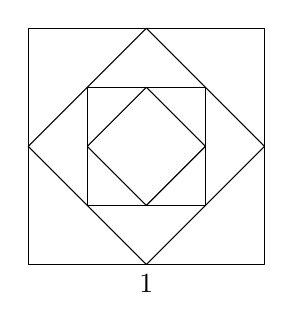
\begin{tikzpicture}[scale=3, line cap=round, line join=round]
	% Hình vuông lớn (cạnh 1)
	\draw (0,0) rectangle (1,1);
	% Hình vuông xoay 45 độ (diamond) bên trong
	\draw (0.5, 0) -- (1, 0.5) -- (0.5, 1) -- (0, 0.5) -- cycle;
	% Hình vuông nhỏ bên trong (cạnh 1/2)
	\draw (0.25,0.25) rectangle (0.75,0.75);
	% Hình vuông nhỏ xoay 45 độ (diamond) bên trong
	\draw (0.5,0.25) -- (0.75,0.5) -- (0.5,0.75) -- (0.25,0.5) -- cycle;
	\node at (0.5,0)[below]{$1$};
	\end{tikzpicture}
	}
	\loigiai{
	Diện tích hình vuông ban đầu là $S_1 = 1^2 = 1$.\\
	Hình vuông thứ hai (tạo bởi nối trung điểm) có cạnh bằng $\dfrac{1}{\sqrt{2}}$ (đường chéo hình vuông nhỏ bằng cạnh hình vuông lớn), nên diện tích là $S_2 = \left(\dfrac{1}{\sqrt{2}}\right)^2 = \dfrac{1}{2}$.\\
	Hình vuông thứ ba có cạnh bằng $\dfrac{1}{2}$, nên diện tích là $S_3 = \left(\dfrac{1}{2}\right)^2 = \dfrac{1}{4}$.\\
	Hình vuông thứ tư có cạnh bằng $\dfrac{1}{2\sqrt{2}}$ nên diện tích $S_4 = \left(\dfrac{1}{2\sqrt{2}}\right)^2=\dfrac{1}{8}$.\\
	Ta thấy dãy diện tích các hình vuông là một cấp số nhân với số hạng đầu $S_1 = 1$ và công bội $q = \dfrac{1}{2}$.\\
	Vậy tổng diện tích của tất cả hình vuông được tạo thành đến lần thứ $ 5 $ là tổng của $ 6 $ số hạng đầu tiên của cấp số nhân trên.
	$$S_6 = u_1\cdot \dfrac{1-q^7}{1 - q} = 1\cdot \dfrac{1-\left(\dfrac{1}{2}\right)^7}{1 - \dfrac{1}{2}} = \dfrac{127}{64}.$$
	}
	\end{ex}
	\begin{ex}[Trích đề thi HKI 11- THPT Hoàng Việt - Đắk Lắk - Năm học 2024-2025]%[1D2C3-8]%[Dự án đề cương 2025]%[Đoàn Minh Tâm]
	Ông Bình cần khoan một cái giếng sau nhà. Biết rằng giá của một mét khoan đầu tiên là $200\,000$ đồng và kể từ mét khoan thứ hai, giá của mỗi mét khoan sau tăng thêm $8\%$ so với giá của mét khoan ngay trước đó. Hỏi nếu khoan $20$ mét thì ông Bình phải trả bao nhiêu tiền? \textit{(kết quả được làm tròn đến hàng đơn vị)}.
	\choice
	{$8\,236\,895$ đồng}{$10\,653\,211$ đồng}{\True $9\,152\,393$ đồng}{$7\,178\,900$ đồng}
	\loigiai{
	Giá tiền khoan $n$ mét là cấp số nhân $u_n$ với số hạng đầu $u_1=200\,000$, công bội $q=108\%=1{,}08$.\\
	Vậy giá tiền khoan $20$ mét là $S_{20}=\dfrac{200\,000\cdot (1-1{,}08^{20})}{1-1{,}08}\approx 9\,152\,393$.
	}
	\end{ex}
\begin{ex}[Trích đề thi HKI 11- THPT Vàm Đình - Cà Mau - Năm học 2024-2025]%[1D2V3-8]%[Dự án đề cương 2025]%[Đoàn Minh Tâm]
	Một loại vi khuẩn sau mỗi phút số lượng tăng gấp đôi biết rằng sau $5$ phút người ta đếm được có $64\,000$ con. Hỏi sau bao nhiêu phút thì có được $8\,192\,000$ con?
	\choice
	{$11$}
	{\True $12$}
	{$26$}
	{$50$}
	\loigiai{
	Số lượng vi khuẩn đã cho theo phút tương ứng tạo thành một cấp số nhân với $u_1$ và công bội $q=2$.\\
	Theo bài ra $u_5=64\, 000\Leftrightarrow u_1\cdot q^4=64\,000\Leftrightarrow u_1 =\dfrac{64\,000}{2^4} =4\,000$.\\
	Do đo $u_n=8\, 192\, 000\Leftrightarrow u_1\cdot q^{n-1} =8\, 192\, 000\Leftrightarrow 2^{n-1} =2048\Leftrightarrow n=12$.\\
	Vậy sau $12$ phút thì số lượng vi khuẩn đạt $8\,192\,000$ con.
	}
\end{ex}

\Closesolutionfile{ans}
	\ind{PHẦN II.} \inden{Câu trắc nghiệm đúng sai. Trong mỗi ý a), b), c), d) ở mỗi câu, học sinh chọn đúng hoặc sai.}\\
\setcounter{ex}{0}
\Opensolutionfile{ans}[ans/1D2-Bai3-DS]%--Đặt tên 2D1-Bai1-DS
\begin{ex}[Trích đề thi HKI 11- THPT Chuyên Lê Hồng Phong - Tp HCM - Năm học 2024-2025]%[1D2V3-4]%[Dự án đề cương 2025]%[Đoàn Minh Tâm]
	Cho dãy số $\left(u_n\right),\left(v_n\right)$ với $\heva{&u_1=2 \\ &u_{n+1}=3u_n-2}$, $v_n=u_n-1$.
	\choiceTF
	{$v_n$ là cấp số nhân với công bội $q=2$}
	{\True $v_n=3^{n-1}$ với mọi $n \geq 1$}
	{\True $v_2=3$}
	{$u_{2024}=3^{2024}+1$}
	\loigiai{
	\begin{itemchoice}
	\itemch \textbf{Sai}. Ta thấy
	$u_{n+1} = 3u_n-2
	\Leftrightarrow u_{n+1}-1 = 3(u_n - 1)
	\Leftrightarrow v_{n+1} = 3v_n$.\\
	Do đó, $(v_n)$ là một cấp số nhân với công bội $q=3$ và $v_1 = u_1 - 1 =2-1=1$.
	\itemch \textbf{Đúng}. Công thức tổng quát của cấp số nhân $(v_n)$
	$$
	v_n = v_1 \cdot q^{n-1} = 3^{n-1} \quad \text{với mọi } n \ge 1.
	$$
	\itemch \textbf{Đúng}. Dễ thấy
	$$
	v_2 = 3^{2-1} = 3.
	$$
	\itemch \textbf{Sai}. Ta có
	$$
	u_n = v_n + 1
	= 3^{n-1} + 1.
	$$
	Suy ra
	$$
	u_{2024} = 3^{2023} + 1.
	$$
	\end{itemchoice}
	}
\end{ex}
\begin{ex}[Trích đề thi HKI 11- THPT Bình Chiểu - TP.HCM - Năm học 2024-2025]%[1D2V3-6]%[Dự án đề cương 2025]%[Đoàn Minh Tâm]
	Cho cấp số nhân $\left(u_n\right)$ thoả mãn $\heva{&u_5-u_2=156\\&u_6-u_3=468.}$
	\choiceTF
	{Số hạng đầu của cấp số nhân bằng $3$}
	{Số hạng thứ $5$ của cấp số nhân bằng $160$}
	{\True Tổng của $12$ số hạng đầu tiên bằng $531\,440$}
	{\True Số $39\,366$ là số hạng thứ $10$ của cấp số nhân}
	\loigiai{Ta có $\heva{&u_5-u_2=156\\&u_6-u_3=468}\Leftrightarrow\heva{&u_1q^4-u_1q=156\\&u_1q^5-u_1q^2=468}\Leftrightarrow\heva{&u_1q\left(q^3-1\right)=156&\quad(1)\\&u_1q^2\left(q^3-1\right)=468.&\quad(2)}$\\
	Lấy $(2)$ chia $(1)$ ta được $q=3$, thay vào $(1)$ ta có $u_1=\dfrac{156}{3\left(3^3-1\right)}=2$.
	\begin{itemchoice}
	\itemch Số hạng đầu của cấp số nhân bằng $2$.
	\itemch Số hạng thứ $5$ của cấp số nhân là $u_5=u_1q^4=2\cdot3^4=162$.
	\itemch Tổng của $12$ số hạng đầu tiên là $S_{12}=u_1\cdot\dfrac{1-q^{12}}{1-q}=2\cdot\dfrac{1-3^{12}}{1-3}=531\,440$.
	\itemch Số hạng thứ $10$ của cấp số nhân là $u_{10}=u_1q^9=2\cdot3^9=39\,366$.
	\end{itemchoice}}
\end{ex}



\begin{ex}%[Dự án đề cương 2025]%[Đoàn Minh Tâm]
 Cho cấp số nhân $\left(u_n\right)$ thoả mãn $\heva{&u_4+u_6=-540 \\ &u_3+u_5=180}$. Khi đó
\choiceTF
{\True Số hạng $u_1=2$ }
{Gọi $q$ là công bội của cấp số nhân, thì ba số $q $; $1 $; $3$ tạo thành một cấp số cộng}
{$-486$ là số hạng thứ $ 5 $ của cấp số nhân}
{\True Tổng của $ 21 $ số hạng đầu cấp số nhân đã cho bằng $ \dfrac{1+3^{21}}{2} $}
\loigiai{
	\begin{itemchoice}
	\itemch \textbf{Sai}. Gọi $q$ là công bội và $S_{21}$ là tổng của $ 21 $ số hạng đầu của cấp số nhân $\left(u_n\right)$.
	\\
	Ta có
	\begin{eqnarray*}
	&&\heva{
	&u_4+u_6=-540 \\ &u_3+u_5=180
	} \\
	&\Leftrightarrow&
	\heva{
	&\left(u_3+u_5\right) q=-540 \\ &u_3+u_5=180
	} \\
	&\Leftrightarrow&
	\heva{
	&180 q=-540 \\ &u_3+u_5=180
	}\\
	&	\Leftrightarrow&
	\heva{
	&q = - 3 \\
	&u _ { 1 } ( - 3 ) ^ { 2 } + u _ { 1 } ( - 3 ) ^ { 4 } = 1 8 0
	} \\
	&\Leftrightarrow &
	\heva{
	&q = - 3 \\
	&u _ { 1 } ( 9 + 8 1 ) = 1 8 0
	} \\
	&\Leftrightarrow&
	\heva{
	&q=-3 \\
	&u_1=2.
	}
	\end{eqnarray*}
	\itemch \textbf{Sai}.	 Gọi $ q $ là công bội của cấp số nhân, thì ba số $ q $; $ 1 $; $ 3 $ tạo thành một cấp số cộng.
	\\
	Với $q=-3$, khi đó ba số $\dfrac{3+(-3)}{2}=0 \neq 1$ không tạo thành một cấp số cộng.
	\itemch \textbf{Sai}.
	Số $-486=2 \cdot(-3)^5$ nên số $ -486 $ là số hạng thứ $ 6 $.
	\itemch \textbf{Đúng}. Ta có $S_{21}=\dfrac{u_1\left(1-q^{21}\right)}{1-q}=\dfrac{2\left[1-(-3)^{21}\right]}{1-(-3)}=\dfrac{1+3^{21}}{2}$.
	\end{itemchoice}
}
\end{ex}
\begin{ex}[Trích đề thi HKI 11- THPT Nguyễn Thị Minh Khai - TP.HCM - Năm học 2024-2025]%[1D2V3-8]%[Dự án đề cương 2025]%[Đoàn Minh Tâm]
	Năm $2023$, một công ty thải ra $125$ tấn rác. Với quyết tâm góp phần giảm thiểu sự ô nhiễm môi trường, công ty quyết định kể từ năm $2024$, mỗi năm phải giảm $5\%$ lượng rác thải so với năm trước đó. Lấy mốc thời gian tính từ năm $2023$ (tức là năm $2023$ được tính là năm thứ nhất), gọi $T_n$ (với $n\in \mathbb{N}^*$) là số tấn rác thải của công ty trong năm thứ $n$.
	\choiceTF
	{\True Số tấn rác thải của công ty trong năm $2024$ là $118{,}75$}
	{Dãy số $(T_n)$ là một cấp số nhân có $T_1=125$ và công bội $q=0{,}05$}
	{\True Công thức số hạng tổng quát của dãy số $(T_n)$ là $T_n=125\cdot(0{,}95)^{n-1}$, với $n\in \mathbb{N}^*$}
	{Nếu điều này được thực hiện thành công thì ước tính trong năm $2038$ khối lượng rác thải của công ty sẽ giảm đi được $50\%$ so với năm $2023$}
	\loigiai{
	Theo bài ra $(T_n)$ là cấp số nhân với $T_1=125$ (tấn) và công bội $q=1-5\%=0{,}95$.\\
	\begin{itemchoice}
	\itemch \textbf{Đúng}.\\
	Khi đó số tấn rác thải của công ty trong năm $2024$ là $T_2=T_1\cdot q=118{,}75$ (tấn).
	\itemch \textbf{Sai}.\\
	Cấp số nhân có công bội $q=0{,}95$.
	\itemch \textbf{Đúng}.\\
	Công thức số hạng tổng quát của dãy số $(T_n)$ là $T_n=125\cdot(0{,}95)^{n-1}$, với $n\in \mathbb{N}^*$.
	\itemch \textbf{Sai}.\\
	Lượng rác thải năm $2038$ là $T_{16}=125\cdot (0{,}95)^{15}\approx 57{,}91$ (tấn).\\
	Phần trăm lượng rác thải giảm đi so với năm $2023$ là khoảng
	$\dfrac{125-57{,}91}{125}\cdot 100\%\approx 53{,}67\%$.
	\end{itemchoice}
	}
\end{ex}
\begin{ex}[Trích đề thi HKI 11- THPT Chuyên Lê Quý Đôn - Ninh Thuận - Năm học 2024-2025]%[1D2C3-8] %[Dự án đề cương 2025]%[Đoàn Minh Tâm]
	Cho hình vuông $(H_1)$ có cạnh bằng $1$. Người ta nối các trung điểm của các cạnh hình vuông này thành hình vuông mới $(H_2)$. Từ hình vuông $(H_2)$ tiếp tục làm như trên ta nhận được dãy hình vuông $(H_1)$, $(H_2)$, $(H_3)$,$\ldots$, $(H_n)$, $\ldots$. Gọi $P_i$ là chu vi của hình vuông $(H_i)$ với $i=1$, $2$, $3$, $\ldots$, $n$, $\ldots$
	\begin{center}
	\begin{tikzpicture}[scale=1, font=\footnotesize,line join=round, line cap=round, >=stealth]
	\coordinate (A) at (0,0);
	\coordinate (B) at (4,0);
	\coordinate (C) at (4,4);
	\coordinate (D) at (0,4);
	\coordinate (E) at ($(A)!0.5!(B)$);
	\coordinate (F) at ($(B)!0.5!(C)$);
	\coordinate (G) at ($(C)!0.5!(D)$);
	\coordinate (H) at ($(D)!0.5!(A)$);
	\coordinate (I) at ($(E)!0.5!(F)$);
	\coordinate (K) at ($(F)!0.5!(G)$);
	\coordinate (L) at ($(G)!0.5!(H)$);
	\coordinate (M) at ($(H)!0.5!(E)$);
	\coordinate (N) at ($(I)!0.5!(K)$);
	\coordinate (O) at ($(K)!0.5!(L)$);
	\coordinate (P) at ($(L)!0.5!(M)$);
	\coordinate (U) at ($(M)!0.5!(I)$);
	\draw (A)--(B)--(C)--(D)--cycle;
	\draw (E)--(F)--(G)--(H)--cycle;
	\draw (I)--(K)--(L)--(M)--cycle;
	\draw (N)--(O)--(P)--(U)--cycle;
	\end{tikzpicture}
	\end{center}
	\choiceTF
	{\True Chu vi $P_2$ của hình vuông $(H_2)$ bằng $2\sqrt{2}$}
	{\True $P_1$, $P_2$, $P_3$, $\ldots$, $P_n$, $\ldots$ lập thành cấp số nhân có cộng bội bằng $\dfrac{1}{\sqrt{2}}$}
	{Chu vi $ P_6 $ của hình vuông $ (H_6) $ bé hơn $ 0{,}5 $ }
	{\True Tổng $P_1+P_2+\ldots+P_{10}=\dfrac{62+31\sqrt{2}}{8}$}
	\loigiai{
	\begin{itemchoice}
	\itemch \textbf{Đúng}.\\
	Hình vuông $(H_2)$ có cạnh bằng $\dfrac{1}{2}$ đường chéo hình vuông $(H_1)$.\\
	Suy ra cạnh của hình vuông $(H_2)$ là $\dfrac{1}{2}\cdot\sqrt{2}=\dfrac{\sqrt{2}}{2}.$\\ $\Rightarrow P_2=4\cdot \dfrac{\sqrt{2}}{2}=2\sqrt{2}$.
	\itemch \textbf{Đúng}.\\
	$P_1=4$.\\
	$P_2=2\sqrt{2}=4\cdot \left(\dfrac{1}{\sqrt{2}}\right)^1$.\\
	$\ldots$\\
	$P_n=4\cdot \left(\dfrac{1}{\sqrt{2}}\right)^{n-1}$.\\
	$\ldots$\\
	Suy ra 	$P_1$, $P_2$, $P_3$, $\ldots$, $P_n$, $\ldots$ lập thành cấp số nhân có cộng bội bằng $\dfrac{1}{\sqrt{2}}$.
	\itemch  \textbf{Sai}.\\
	Ta có  $ P_6=P_1\cdot \left(\dfrac{1}{\sqrt{2}}\right)^5=\dfrac{\sqrt{2}}{2} >0{,}5 $.
	\itemch \textbf{Đúng}.\\
	Do $P_1$, $P_2$, $P_3$, $\ldots$, $P_n$, $\ldots$ lập thành cấp số nhân có cộng bội bằng $\dfrac{1}{\sqrt{2}}$. \\
	Nên $P_1+P_2+\cdots+P_{10}=4\cdot\dfrac{1-\left(\dfrac{1}{\sqrt{2}}\right)^{10}}{1-\dfrac{1}{\sqrt{2}}}=\dfrac{62+31\sqrt{2}}{8}$.
	\end{itemchoice}
	}
\end{ex}
\Closesolutionfile{ans}
\ind{PHẦN III.} \inden{Câu trắc nghiệm trả lời ngắn}\\
\setcounter{ex}{0}
\Opensolutionfile{ans}[ans/1D2-Bai3-TLN]
\begin{ex}%[Dự án đề cương 2025]%[Đoàn Minh Tâm]
	Ba số $x$, $y$, $z$ theo thứ tự lập thành một cấp số cộng tăng có tổng bằng $24$. Nếu cộng thêm lần lượt các số $1$, $4$, $13$ vào ba số $x$, $y$, $z$ ta được ba số theo thứ tự lập thành cấp số nhân. Tính giá trị biểu thức $P=x^2+y^2+z^2$.
	\shortans[oly]{$ 210 $}
	\loigiai{
	Ba số $x$, $y$, $z$ theo thứ tự lập thành một cấp số cộng có tổng bằng $24$ nên ta có hệ phương trình
	$$
	\heva{&	x+y+z=24 \\
	&x+z=2 y
	}\Rightarrow 3 y=24 \Rightarrow y=8.
	$$
	Ta viết lại $3$ số $x$, $y$, $z$ lần lượt bằng $8-d$, $8$, $8+d$.
	Nếu cộng thêm lần lượt các số $1$, $4$, $13$ vào ba số $x$, $y$, $z$ ta được ba số là $9-d$, $12$, $21+d$.
	\\
	Vì ba số này theo thứ tự lập thành cấp số nhân nên ta có phương trình:
	$$(9-d)(21+d)=12^2 	\Leftrightarrow d^2+12 d-45=0 \Leftrightarrow	\hoac{
	&d=3 \\
	&d=-15
	}
	$$
	Vì cấp số cộng tăng nên $d>0 \Rightarrow d=3 \Rightarrow$ ba số $x$, $y$, $z$ lần lượt bằng $5$, $8$, $11$.
	\\
	Suy ra $P=x^2+y^2+z^2=5^2+8^2+11^2=210$.
	}
\end{ex}
\begin{ex}[Trích đề thi HKI 11- THPT Phan Bội Châu - Lâm Đồng - Năm học 2024-2025]%[1D2V3-8]%[Dự án đề cương 2025]%[Đoàn Minh Tâm]
	Một du khách vào trường đua ngựa xem đua ngựa và đặt cược chọn con thắng cuộc. Nếu chọn đúng con thắng cuộc thì sẽ nhận được số tiền gấp đôi số tiền đặt cược, còn nếu chọn sai thì sẽ mất số tiền đặt cược. Người du khách đó lần đầu tiên đặt $100$ USD , mỗi lần sau tiền đặt gấp đôi tiền đặt lần trước. Người đó thua $9$ lần liên tiếp và thắng ở lần thứ $10$. Sau $10$ lần chơi, du khách đó đã lời được $a$ USD. Hãy tìm $a$.
	\shortans[oly]{$100$}
	\loigiai{
	\textbf{\textit{Cách 1:}}\\
	Tổng số tiền đã thua trong $9$ lần đầu tiên là tổng của một cấp số nhân với số hạng đầu $u_1 = 100$, công bội $q = 2$.\\
	Vậy, tổng số tiền thua là $S_9 = \dfrac{100\cdot (2^9 - 1)}{2 - 1} = \dfrac{100\cdot (512 - 1)}{1} = 100\cdot 511 = 51\,100$ USD.\\
	Ở lần thứ $10$, người du khách đặt số tiền là $u_{10}=u_1\cdot 2^9=51\,200$.\\
	Ở lần thứ $10$, người du khách thắng và nhận được số tiền gấp đôi số tiền đặt cược là $51\,200\cdot 2 = 102\,400$ USD.\\
	Số tiền lời ở lần thắng này so với số tiền đã đặt là $102\,400 - 51\,200 = 51\,200$ USD.\\
	Vậy, sau $10$ lần chơi, du khách đó đã lời được $51\,200 - 51\,100 =100$ USD.\\
	\textbf{\textit{Cách 2:}}\\
	Ta sẽ tính số tiền đặt cược và kết quả của từng lần chơi:
	\begin{itemize}
	\item Lần 1: Đặt cược $100$ USD, thua. Số tiền mất là $100$ USD.
	\item Lần 2: Đặt cược $100\cdot 2 = 200$ USD, thua. Số tiền mất là $200$ USD.
	\item Lần 3: Đặt cược $200\cdot 2 = 400$ USD, thua. Số tiền mất là $400$ USD.
	\item Lần 4: Đặt cược $400\cdot 2 = 800$ USD, thua. Số tiền mất là $800$ USD.
	\item Lần 5: Đặt cược $800\cdot 2 = 1\,600$ USD, thua. Số tiền mất là $1\,600$ USD.
	\item Lần 6: Đặt cược $1\,600\cdot 2 = 3\,200$ USD, thua. Số tiền mất là $3\,200$ USD.
	\item Lần 7: Đặt cược $3\,200\cdot 2 = 6\,400$ USD, thua. Số tiền mất là $6\,400$ USD.
	\item Lần 8: Đặt cược $6\,400\cdot 2 = 12\,800$ USD, thua. Số tiền mất là $12\,800$ USD.
	\item Lần 9: Đặt cược $12\,800\cdot 2 = 25\,600$ USD, thua. Số tiền mất là $25\,600$ USD.
	\item Lần 10: Đặt cược $25600\cdot 2 = 51200$ USD, thắng. Số tiền nhận được là $51200\cdot 2 = 102400$ USD.\\
	Số tiền lời ở lần thắng này so với số tiền đã đặt là $102\,400 - 51\,200 = 51200$ USD.
	\end{itemize}
	Vậy, sau $10$ lần chơi, du khách đó đã lời được $51\,200 - 51\,100 =100$ USD.
	}
\end{ex}
\begin{ex}[Trích đề thi HKI 11- THPT Lê Quý Đôn - TPHCM - Năm học 2024-2025]%[1D2V3-3]%[Dự án đề cương 2025]%[Đoàn Minh Tâm]
	Một công ty mua một cái máy với giá $1$ tỉ $800$ triệu đồng. Công ty nhận thấy, trong vòng $5$ năm đầu, tốc độ khấu hao là $25\%$ trên một năm (tức là sau mỗi một năm, giá trị còn lại của chiếc máy bằng $75\%$ giá trị của năm trước đó). Sau $5$ năm, giá trị của cái máy đó còn khoảng bao nhiêu triệu đồng (làm tròn kết quả đến hàng đơn vị)?
	\shortans[oly]{$427$}
	\loigiai{Sau một năm giá trị còn lại của một cái máy là $u_1=1\,800\cdot \dfrac{3}{4}$.\\
	Quy luật này xác định một cấp số nhân có $q=\dfrac{3}{4}$.\\
	Sau $5$ năm, giá trị của cái máy còn lại là $u_5=1\,800\cdot \left( \dfrac{3}{4}\right)^5=\dfrac{54675}{128}\approx 427$ triệu đồng.
	}
\end{ex}
\begin{ex}[Trích đề thi HKI 11- THPT Chuyên Hùng Vương - Phú Thọ - Năm học 2024-2025]%[1D2V3-8]%[Dự án đề cương 2025]%[Đoàn Minh Tâm]
	Theo thống kê của Chi cục Dân số Hà Nội, tính đến năm $2024$, dân số thủ đô Hà Nội ước tính đạt khoảng $8{,}5$ triệu người và tốc độ tăng trưởng dân số là $1{,}26\%$. Nếu tốc độ tăng trưởng dân số này được giữ nguyên hàng năm, hãy ước tính dân số của thủ đô Hà Nội vào năm $2030$ (tính theo đơn vị triệu người, làm tròn đến hàng phần trăm).
	\shortans[oly]{$9{,}16$}
	\loigiai{
	Theo giả thuyết đề bài, dân số thủ đô Hà Nội qua các năm là một cấp số nhân với $u_1=8{,}5$ và $q=1{,}26\%$.\\
	Dân số $2030$ là số hạng thứ $7$ của cấp số nhân trên. Do đó,
	$$u_7=u_1\cdot q^6=8{,}5\cdot \left(1+1{,}26\%\right)^6\approx 9{,}16.$$
	}
\end{ex}
\begin{ex}[Trích đề thi HKI 11- THPT Nguyễn Gia Thiều - Hà Nội- Năm học 2024-2025]%[1D2V3-6]%[Dự án đề cương 2025]%[Đoàn Minh Tâm]
	Anh An kí hợp đồng lao động $5$ năm và được trả lương như sau: Tháng thứ nhất tiền lương là $16$ triệu đồng, kể từ tháng thứ hai trở đi mỗi tháng tiền lương được tăng lên $1$\%. Anh An đã lên kế hoạch quản lý tài chính cá nhân như sau: Ngay từ tháng lương đầu tiên, hàng tháng chuyển tiết kiệm vào tài
	khoản đúng bằng $30$\% tiền lương của tháng đó, biết lãi suất trong tài khoản nhỏ coi như không có. Hỏi anh An cần tối thiểu bao nhiêu tháng kể từ tháng lương đầu tiên để tiền tiết kiệm này đủ mua chiếc xe máy giá $120$ triệu đồng mà không phải vay mượn ai?
	\shortans[oly]{$23$}
	\loigiai{
	Tiền lương ở tháng thứ $n$ là $L_n=16\cdot 1{,}01^{n-1}$ (triệu đồng).\\
	Tiền tiết kiệm ở tháng thứ $n$ là $T_n=0{,}3\cdot L_n=0{,}3\cdot 16\cdot 1{,}01^{n-1}=4{,}8\cdot 1{,}01^{n-1}$ (triệu đồng).\\
	Tổng số tiền tiết kiệm sau $n$ tháng là
	\begin{center}
	$S_n=T_1+T_2+\cdots+T_n=4{,}8\cdot \dfrac{(1{,}01)^n-1}{1{,}01-1}=480\left[(1{,}01)^n-1\right]$ (triệu đồng).
	\end{center}
	Ta có
	\begin{eqnarray*}
	S_n\ge 120&\Leftrightarrow& 480\left[(1{,}01)^n-1\right]\ge 120\\
	&\Leftrightarrow& (1{,}01)^n\ge 1{,}25\\
	&\Leftrightarrow& n\ge \log_{1{,}01}1{,}25\\
	&\Rightarrow& n\ge 22{,}4.
	\end{eqnarray*}
	Vậy anh An cần tối thiểu $23$ tháng để có đủ tiền mua xe.
	}
\end{ex}
\begin{ex}[Trích đề thi HKI 11- THPT Phan Bội Châu - Bình Thuận - Năm học 2024-2025]%[1D2V3-8]%[Dự án đề cương 2025]%[Đoàn Minh Tâm]
	Một loại vi khuẩn sinh sản thông qua một quá trình gọi là quá trình phân đôi. (Quá trình phân đôi ở vi khuẩn xảy ra hiện tượng gấp nếp màng sinh chất tạo ra mêzôxôm – cấu trúc có vai trò làm điểm tựa cho vòng ADN nhân đôi đồng thời góp phần hình thành nên vách ngăn phân chia tế bào mẹ thành hai tế bào con). Nếu trong điều kiện nuôi cấy thích hợp thì cứ sau một phút lại phân đôi một lần. Biết rằng sau $5$ lần phân chia người ta đếm được có $64\,000$ con. Hỏi sau bao nhiêu phút thì có được $2\,048\,000$ con?
	\shortans[oly]{$10$}
	\loigiai{
	Gọi $u_1$ là số con vi khuẩn ban đầu và mỗi lần phân chia thành hai con nên ta có cấp số nhân với công bội $q=2$ và $u_6$ là số vi khuẩn nhận được sau $5$ lần phân chia.\\
	Ta có $u_6=64\,000\Rightarrow{u_1}\cdot q^5=64\,000\Rightarrow{u_1}=2\,000$.\\
	Sau $n$ phút thì số lượng vi khuẩn là $u_{n+1}$ nên
	\begin{eqnarray*}
	&&u_{n+1}=2\,048\,000\\
	&\Leftrightarrow& u_1\cdot q^n=204\,8000\\
	&\Leftrightarrow& 2\,000\cdot 2^n=2\,048\,000\Rightarrow n=10.
	\end{eqnarray*}
	Vậy sau $10$ phút thì có được $2\,048\,000$ con.}
\end{ex}
\begin{ex}%[Dự án đề cương 2025]%[Đoàn Minh Tâm]
	Có bao nhiêu giá trị nguyên của tham số $m$ để phương trình sau có ba nghiệm phân biệt lập thành một cấp số nhân $x^3-7 x^2+2\left(m^2+6 m\right) x-8=0$.
	\shortans[oly]{$ 2 $}
	\loigiai{
	\begin{itemize}
	\item 	\textbf{Điều kiện cần:} Giả sử phương trình đã cho có ba nghiệm phân biệt $x_1$, $x_2$, $x_3$ lập thành một cấp số nhân.
	\\
	Ta có: $x^3-7 x^2+2\left(m^2+6 m\right) x-8=\left(x-x_1\right)\left(x-x_2\right)\left(x-x_3\right), \forall m \in R \Rightarrow x_1 x_2 x_3=8$.
	\\
	Theo tính chất của cấp số nhân: $x_1 x_3=x_2^2$.
	\\
	Suy ra $x_2^3=8 \Rightarrow x_2=2$.
	\\
	Thay nghiệm $x=x_2=2$ vào phương trình đã cho, ta có
	$$
	8-28+2\left(m^2+6 m\right) \cdot 2-8=0 \Leftrightarrow 4 m^2+24 m-28=0
	\Leftrightarrow
	\hoac{
	&m=1 \\
	&	m=-7
	}
	$$
	\item 	\textbf{Điều kiện đủ:} Thử lại với các giá trị m tìm được.
	\begin{itemize}
	\item Với $m=1$, ta có phương trình: $x^3-7 x^2+14 x-8=0 \Leftrightarrow
	\hoac{
	&x=4 \\ &x=2 \\ &x=1
	}$ (thoả mãn).
	\item Với $m=-7$, ta có phương trình $x^3-7 x^2+14 x-8=0 \Leftrightarrow
	\hoac{
	&x=4 \\ &x=2 \\ &x=1
	}$ (thoả mãn).
	\end{itemize}
	Vậy $m=1 ; m=-7$ là các giá trị cần tìm.
	\end{itemize}
	}
\end{ex}
\Closesolutionfile{ans}
\ind{PHẦN IV.} \inden{Tự luận.}\\
\setcounter{ex}{0}
\Opensolutionfile{ans}[ans/1D2-Bai3-TL]%--Đặt tên 2D1-Bai1-DS
\begin{ex}%[Dự án đề cương 2025]%[Đoàn Minh Tâm]
	Cho cấp số nhân $\left(u_n\right)$ có $S_2=4$ và $S_3=13$ (trong đó $S_2, S_3$ theo thứ tự là tổng của hai và của ba số hạng đầu của cấp số nhân). Tổng của năm số hạng đầu của cấp số nhân có công bội dương có giá trị bằng bao nhiêu?
	\loigiai{
	Ta có: $u_3=S_3-S_2=9 \Rightarrow u_1 q^2=9 \Rightarrow u_1=\dfrac{9}{q^2} \quad (1)$ (vì $q \neq 0$ ).
	\\
	Mặt khác $S_2=4$ nên $u_1+u_1 q=4 \quad (2)$.
	\\
	Thay (1) vào (2), ta có $\dfrac{9}{q^2}+\dfrac{9}{q}=4 \Leftrightarrow 4 q^2-9 q-9=0 \Leftrightarrow q=3$ hoặc $q=-\dfrac{3}{4}$.
	\\
	Với $q=3$ thì $u_1=1$, khi đó
	$
	S_5=\dfrac{u_1\left(1-q^5\right)}{1-q}=\dfrac{1\left(1-3^5\right)}{1-3}=121.
	$
	}
\end{ex}
%\Closesolutionfile{ans}
\begin{ex}%[Dự án đề cương 2025]%[Đoàn Minh Tâm]
	Có bao nhiêu giá trị của $x$ để các số $2 x-1 $; $x $; $2 x+1$ theo thứ tự lập thành một cấp số nhân.
	\loigiai{
	Vì $2 x-1 $; $x $; $2 x+1$ theo thứ tự lập thành cấp số nhân
	$\Rightarrow(2 x-1)(2 x+1)=x^2 \Rightarrow 4 x^2-1=x^2 \Rightarrow x= \pm \dfrac{1}{\sqrt{3}}$.
	\\
	Vậy có hai giá trị $x= \pm \dfrac{1}{\sqrt{3}}$ thoả mãn đề bài.
	}
\end{ex}
\begin{ex}%[Dự án đề cương 2025]%[Đoàn Minh Tâm]
	Cho các số $x+6 y $; $5 x+2 y $; $8 x+y$ theo thứ tự lập thành một cấp số cộng; đồng thời các số $x-1 $; $y+2 $; $x-3 y$ theo thứ tự đó lập thành một cấp số nhân. Tính $x^2+y^2$.
	\loigiai{
	Theo giả thiết, ta có:
	$\heva{
	&(x+6 y)+(8 x+y)=2(5 x+2 y) \\ &(x-1)(x-3 y)=(y+2)^2}
	\Leftrightarrow
	\heva{
	&x = 3 y \\
	&( 3 y - 1 ) ( 3 y - 3 y ) = ( y + 2 ) ^ { 2 }
	y}
	\Leftrightarrow
	\heva{
	&x = 3 y \\
	&0 = ( y + 2 ) ^ { 2 }
	}
	\Leftrightarrow
	\heva{
	&x=-6 \\
	&y=-2.
	}
	$\\
	Suy ra $x^2+y^2=40$.
	}
\end{ex}
\begin{ex}%[Dự án đề cương 2025]%[Đoàn Minh Tâm]
	Kết quả của tổng $S=1+2 \cdot 5+3 \cdot 5^2+\cdots+79 \cdot 5^{78}$ được viết dưới dạng $a+\dfrac{315}{16} \cdot 5^b$ ($b \in \mathbb{N}$, $a$ là phân số tối giản). Tính giá trị biểu thức $P=a+\dfrac{b}{16}$.
	\loigiai{
	Từ giả thiết, ta có $5 S=5+2 \cdot 5^2+3 \cdot 5^3+\ldots+79 \cdot 5^{79}$.
	\\
	Do đó, $-4 S=S-5 S=\underbrace{1+5+5^2+\ldots+5^{78}}_{S'}-79\cdot 5^{79}$.
	\\
	Xét tổng $S'=1+5+5^2+\cdots+5^{78}$ là tổng của $ 79 $ số hạng của một cấp số nhân có số hạng đầu bằng $ 1 $ và công bội bằng $ 5 $, ta có $S'=\dfrac{1-5^{79}}{1-5}$.
	\\
	Vậy $-4 S=S'-79 \cdot 5^{79}=\dfrac{1-5^{79}}{1-5}-79 \cdot 5^{79}=-\dfrac{1}{4}-\dfrac{315 \cdot 5^{79}}{4} \Rightarrow S=\dfrac{1}{16}+\dfrac{315}{16} \cdot 5^{79}$.
	\\
	Ta có $S=\dfrac{1}{16}+\dfrac{315}{16} \cdot 5^{79}=a+\dfrac{315}{16} \cdot 5^b \Rightarrow a=\dfrac{1}{16}$, $b=79 \Rightarrow P=\dfrac{1}{16}+\dfrac{79}{16}=5$.
	}
\end{ex}
\begin{ex}[Trích đề thi HKI 11- THPT Mạc Đĩnh Chi - Năm học 2024-2025]%[1D2H3-8]%[Dự án đề cương 2025]%[Đoàn Minh Tâm]
	Một loại lợi khuẩn được nuôi cấy trong phòng thí nghiệm, cứ sau hai phút số lượng lợi khuẩn lại tăng lên gấp đôi so với số lượng đang có. Từ $ 1$ lợi khuẩn ban đầu, hãy tính tổng số lợi khuẩn có trong ống nghiệm sau $ 28$ phút.
	\loigiai{
	Thời gian $ 28 $ phút tương ứng trải qua $\dfrac{28}{2}=14$ lần nhân đôi.\\
	Do đó, sau $ 28 $ phút, tổng số lợi khuẩn có trong ống nghiệm là $1\cdot 2^{14}=16\,384$.
	}
\end{ex}
\begin{ex}[Trích đề thi HKI 11- Sở Giáo dục tỉnh Bắc Ninh - Năm học 2024-2025]%[1D2V3-8]%[Dự án đề cương 2025]%[Đoàn Minh Tâm]
	Một khay nước có nhiệt độ $29^\circ$C được đặt vào trong tủ lạnh. Biết rằng sau mỗi giờ, nhiệt độ của nước giảm $20\%$.
	\begin{enumerate}
	\item Gọi $u_n$ là nhiệt độ của khay nước đó sau $n$ ($n \in \mathbb{N}^*$) giờ theo đơn vị độ C. Tìm $u_n$.
	\item Tính nhiệt độ của khay nước đó sau $ 8 $ giờ theo đơn vị độ C, làm tròn đến hàng đơn vị.
	\end{enumerate}
	\loigiai{
	\begin{enumerate}
	\item Nhiệt độ của khay nước sau $1$ giờ là $u_1 = 29 \cdot (1-0{,}2)$ ($^\circ$C). \\
	Nhiệt độ của khay nước sau $2$ giờ là $u_ 2= u_1 \cdot (1-0{,}2) = 29\cdot (1-0{,}2)^2$ ($^\circ$C). \\
	Nhiệt độ của khay nước sau $3$ giờ là $u_ 3= u_2 \cdot (1-0{,}2) = 29\cdot (1-0{,}2)^3$ ($^\circ$C). \\
	\ldots\\
Như vậy, ta thấy được nhiệt độ của khay nước là một cấp số nhân có $ u_1=29 \cdot (1-0{,}2) $ với công bội là $ (1-0{,}2) $.\\
Vậy sau $n$ giờ, tức là
 $$u_n = 29 \cdot (1-0{,}2)^n \text{ ($^\circ$C)}.$$
	\item Nhiệt độ của khay nước sau $ 8 $ giờ là $u_8 = 29 \cdot (1-0{,}2)^8 \approx 5$ ($^\circ$C).
	\end{enumerate}
	}
\end{ex}
\begin{ex}[Trích đề thi HKI 11- Chuyên Lê Hồng Phong - Tp HCM - Năm học 2024-2025]%[1D2H3-8]%[Dự án đề cương 2025]%[Đoàn Minh Tâm]
	Một người ký hợp đồng với một công ty theo thỏa thuận: Năm đầu tiên người đó nhận mức lương $ 12 $ triệu đồng mỗi tháng, từ năm thứ hai trở đi mức lương hàng tháng của mỗi năm được tăng $12\%$ so với mức lương hàng tháng của năm trước đó. Hỏi sau $5$ năm, tổng số tiền người đó nhận được là bao nhiêu triệu đồng (làm tròn kết quả tới hàng đơn vị)?
	\loigiai{
	Năm đầu tiên người đó nhận mức lương $12$ triệu đồng mỗi tháng nên tổng tiền lương năm đầu tiên là $T=12 \cdot 12= 144$ (triệu đồng). Suy ra $u_1=144$.\\
	Do từ năm thứ hai trở đi, mức lương hàng tháng của mỗi năm được tăng $12\%$ so với mức lương hàng tháng của năm trước đó nên $q=1+12\%=1{,}12$.\\
	Như vậy sau $5$ năm, người đó có được tổng số tiền lương là
	$$S_5=\dfrac{u_1 \cdot \left(1-q^5\right)}{1-q}=\dfrac{144\left(1-1{,}12^5\right)}{1-1{,}12}\approx 915 \text{ triệu đồng}.$$
	}
\end{ex}
\begin{ex}[Trích đề thi HKI 11- THPT Chuyên Lê Quý Đôn - Ninh Thuận - Năm học 2024-2025]%[1D6H3-5]%[Dự án đề cương 2025]%[Đoàn Minh Tâm]
	Tính đến tháng $12$ năm $2\,024$, dân số Việt Nam khoảng $99{,}77$ triệu người. Nếu tỉ lệ tăng dân số mỗi năm đều bằng $0{,}97\%$ thì vào tháng $12$ năm $2\,034$ dân số Việt Nam khoảng bao nhiêu triệu người? (Kết quả làm tròn đến hàng đơn vị)
	\loigiai{
	Dân số Việt Nam năm $2\,025$ là $S_1=99{,}77+99{,}77\cdot 0{,}97\%=99{,}77\cdot\left(1+0{,}97\%\right)$.\\
	Dân số Việt Nam năm $2\,026$ là
	\begin{eqnarray*}
	&S_2&99{,}77\cdot\left(1+0{,}97\%\right) + 99{,}77\cdot\left(1+0{,}97\%\right)\cdot0{,}97\%\\
	&=&99{,}77\cdot\left(1+0{,}97\%\right)^2.
	\end{eqnarray*}
	Dân số Việt Nam năm $2\,026$ là \allowdisplaybreaks
	\begin{eqnarray*}
	&S_3&99{,}77\cdot\left(1+0{,}97\%\right)^2+99{,}77\cdot\left(1+0{,}97\%\right)^2\cdot 0{,}97\%\\
	&=&99{,}77\cdot\left(1+0{,}97\%\right)^3.
	\end{eqnarray*}
	Ta thấy đây là dãy cấp số nhân với công bội là $q=1+0{,}97\%$.\\
	Nên tổng dân số Việt Nam vào tháng $ 12 $ năm $2\,034$ là \allowdisplaybreaks
	\begin{eqnarray*}
	S&=&99{,}77\cdot\left(1+0{,}97\%\right)\cdot\dfrac{1-\left(1+0{,}97\%\right)^{10}}{1-\left(1+0{,}97\%\right)}\\
	&\approx& 1\,053.
	\end{eqnarray*}
	Vậy dân số Việt Nam vào tháng $12$ năm $2\,034$ khoảng $1\,053$ triệu người.}
\end{ex}
\begin{ex}[Trích đề thi HKI 11- THPT Bắc Yên Thành - Nghệ An - Năm học 2024-2025]%[1D2V3-8]%[Dự án đề cương 2025]%[Đoàn Minh Tâm]
	Để tích lũy tiền cho chi phí học đại học của con gái, cô Hoa quyết định đầu mỗi tháng gửi $500$ nghìn đồng vào tài khoản tiết kiệm ngân hàng với lãi suất theo tháng là $0{,}5\%$ , tiền lãi hàng tháng được cộng vào tiền gốc. Hỏi cô ấy tích lũy được bao nhiêu tiền vào thời điểm gửi khoản tiền lần thứ $180$ (vào đầu
	tháng thứ $180$)?
	\loigiai{
	Gọi $u_n$ là số triệu đồng mà cô Hoa tích luỹ được vào thời điểm gửi khoản tiền thứ (vào đầu tháng thứ $n$).\\
	Kí hiệu $a=0,5$ triệu đồng, $r=0{,}5 \%$.\\
	Số tiền của cô Hoa tích luỹ được vào thời điểm đầu tháng thứ 1 là $u_1=a$.\\
	Số tiền của cô Hoa tích luỹ được vào thời điểm đầu tháng thứ 2 là
	$$u_2=u_1(1+r)+a=a(1+r)+a.$$
	Số tiền của cô Hoa tích luỹ được vào thời điểm đầu tháng thứ 3 là
	$$u_3=u_2(1+r)+a=a(1+r)^2+a(1+r)+a .$$
	Tương tự cho các tháng tiếp theo, suy ra số tiền của cô Hoa trong chương trình ở đầu tháng thứ $n$ là
	$$
	u_n=a(1+r)^{n-1}+a(1+r)^{n-2}+\ldots+a(1+r)+a=a \dfrac{(1+r)^n-1}{(1+r)-1}=a \dfrac{(1+r)^n-1}{r}.
	$$
	Vào thời điểm gửi khoản tiền thứ $ 180 $, cô ấy sẽ tích luỹ được $$u_{180}=a \dfrac{(1+r)^{180}-1}{r}=145{,}41 \text{ (triệu đồng)}.$$
	}
\end{ex}
\begin{ex}%[1D2C3-4]%[Dự án đề cương 2025]%[Đoàn Minh Tâm]
	Cho cấp số nhân $(u_n)$ có $u_1=3$ và $15 u_1-4 u_2+u_3$ đạt giá trị nhỏ nhất. Tìm số hạng thứ $10$ của cấp số nhân đã cho.
	\shortans{$1536$}
	\loigiai{
		Gọi $q$ là công bội của cấp số nhân $(u_n)$.\\
		Ta có $u_2=u_1 q=3 q $; $u_3=u_1 q^2=3 q^2$.\\
		Suy ra $15 u_1-4 u_2+u_3=45-12 q+3 q^2=3(q-2)^2+33 \geq 33$, $\forall q \in \mathbb{R}$.\\
		Ta có:$15 u_1-4 u_2+u_3$ đạt giá trị nhỏ nhất (bằng $ 33 $) khi và chỉ khi ${q=2}$.\\
		Khi đó $u_{10}=u_1 q^{9}=3 \cdot 2^{9}=1\,536$.
	}
\end{ex}
\Closesolutionfile{ans}